\chapter{Low-rank NMF model for RIR spectrogram}
\label{chapter:trans2020}

\section{Justification of low-rank approximation}
\begin{itemize}
\item Quality of approximation
\item generalization of separability approximation
\begin{itemize}
\item remove limitations of earlier work
\item easy to interpret model
\end{itemize}
\end{itemize}

\section{NMF model for degraded spectrogram}
\begin{itemize}
\item derivation of NMF model for reverb and degraded spectrogram
\item comparison of degradation model obtained with proposed method when compared with NMF based methods in literature
\item effect of clean speech bases and activation with reverberation
\end{itemize}

\section{Algorithm details}
\begin{itemize}
\item cost function
\item multiplicative update rule
\end{itemize}

\section{Experimental results}
\begin{itemize}
\item enhancement results, ASR results
\item variation of performance with RIR, SNR, rank of decomposition, etc.
\end{itemize}

\begin{table}[]
\centering
\begin{tabular}{|l|c|}
\hline
\multicolumn{1}{|c|}{\textbf{Method}} & \textbf{WER (\%)} \\ \hline
Clean                                 & 3.44              \\ \hline
Degraded                              & 62.34             \\ \hline
CNMF0                                 & 47.95             \\ \hline
CNMF1\_s                              & 44.45             \\ \hline
CNMF2\_s                              & 43.24             \\ \hline
RNMF\_s                               & \textbf{40.24}    \\ \hline
\end{tabular}
\caption{Enhancement results when reverberated with RIR \text{RIR3\_far} and stationary noise added with $10$~dB SNR. The RIR has $T_{60}\approx 700$~ms and source-microphone distance of $2$~m. }
\end{table}

\begin{table}[]
\centering
\begin{tabular}{|l|c|l|l|l|}
\hline
\multicolumn{1}{|c|}{\textbf{Method}}                                                         & \multicolumn{4}{c|}{\textbf{WER (\%)}}                                                                                                     \\ \hline
Clean                                                                                         & \multicolumn{4}{c|}{3.44}                                                                                                                  \\ \hline
\multirow{2}{*}{\textbf{\begin{tabular}[c]{@{}l@{}}Degradation \\ condition\end{tabular}}} & \textbf{R2\_near} & \multicolumn{1}{c|}{\textbf{R2\_far}} & \multicolumn{1}{c|}{\textbf{R3\_near}} & \multicolumn{1}{c|}{\textbf{R3\_far}} \\ \cline{2-5} 
                                                                                              &                   & \multicolumn{1}{c|}{48.57}            & \multicolumn{1}{c|}{19.41}             & \multicolumn{1}{c|}{62.34}            \\ \hline
CNMF0                                                                                         &                   &                                       &                                        & 47.95                                 \\ \hline
CNMF1\_s                                                                                      &                   &                                       &                                        & 44.45                                 \\ \hline
CNMF2\_s                                                                                      &                   &                                       &                                        & 43.24                                 \\ \hline
RNMF\_s                                                                                       &                   &                                       &                                        & \textbf{40.24}                        \\ \hline
\end{tabular}
\caption{Enhancement results for $10$~dB SNR stationary noise.}
\end{table}

\begin{table}[]
\centering
\begin{tabular}{|l|c|l|l|l|}
\hline
\multicolumn{1}{|c|}{\textbf{Method}}                                                         & \multicolumn{4}{c|}{\textbf{WER (\%)}}                                                                                                     \\ \hline
Clean                                                                                         & \multicolumn{4}{c|}{3.44}                                                                                                                  \\ \hline
\multirow{2}{*}{\textbf{\begin{tabular}[c]{@{}l@{}}Degradation \\ condition\end{tabular}}} & \textbf{R2\_near} & \multicolumn{1}{c|}{\textbf{R2\_far}} & \multicolumn{1}{c|}{\textbf{R3\_near}} & \multicolumn{1}{c|}{\textbf{R3\_far}} \\ \cline{2-5} 
                                                                                              &                   & \multicolumn{1}{c|}{}            & \multicolumn{1}{c|}{}             & \multicolumn{1}{c|}{}            \\ \hline
CNMF0                                                                                         &                   &                                       &                                        &                                  \\ \hline
CNMF1\_s                                                                                      &                   &                                       &                                        &                                  \\ \hline
CNMF2\_s                                                                                      &                   &                                       &                                        &                                  \\ \hline
RNMF\_s                                                                                       &                   &                                       &                                        &                         \\ \hline
\end{tabular}
\caption{Enhancement results for $20$~dB SNR stationary noise.}
\end{table}

\begin{table}[]
\centering
\begin{tabular}{|l|c|l|l|l|}
\hline
\multicolumn{1}{|c|}{\textbf{Method}}                                                         & \multicolumn{4}{c|}{\textbf{WER (\%)}}                                                                                                     \\ \hline
Clean                                                                                         & \multicolumn{4}{c|}{3.44}                                                                                                                  \\ \hline
\multirow{2}{*}{\textbf{\begin{tabular}[c]{@{}l@{}}Degradation \\ condition\end{tabular}}} & \textbf{R2\_near} & \multicolumn{1}{c|}{\textbf{R2\_far}} & \multicolumn{1}{c|}{\textbf{R3\_near}} & \multicolumn{1}{c|}{\textbf{R3\_far}} \\ \cline{2-5} 
                                                                                              &                   & \multicolumn{1}{c|}{}            & \multicolumn{1}{c|}{}             & \multicolumn{1}{c|}{}            \\ \hline
CNMF0                                                                                         &                   &                                       &                                        &                                  \\ \hline
CNMF1\_s                                                                                      &                   &                                       &                                        &                                  \\ \hline
CNMF2\_s                                                                                      &                   &                                       &                                        &                                  \\ \hline
RNMF\_s                                                                                       &                   &                                       &                                        & \textbf{}                        \\ \hline
\end{tabular}
\caption{Enhancement results for noise free condition.}
\end{table}

\section{Discussion}

\iffalse
\section{Introduction}
Speech originating from a source undergoes multiple reflections in a closed room. When this speech is captured using a microphone distant from the source (typically 30 cm to few meters), the microphone output is a superposition of the speech along with the delayed and attenuated copies of the signal referred to as reverberated speech~\cite{naylor2010speech}. Additionally, the microphone will capture background noise originating from other sources. The resulting microphone output in such a distant speech recording (DSR) setting is a degraded version of the original speech signal. The presence of such degradations impedes speech intelligibility~\cite{kinoshita2016summary}  and automatic speech recognition (ASR)~\cite{barker2018fifth, barker2015third} performance. The amount of degradation depends on the source and microphone positions, characteristics of the room and the noise~\cite{naylor2010speech,kinoshita2016summary}. To improve performance, it is desirable to compensate for these degradations. The focus of this work is on jointly handling dereverberation and denoising. In this work we refer to methods that perform dereverberation in presence of noise as speech enhancement methods.

Dereverberation methods in literature can be broadly classified as (i) beamforming methods, (ii) inverse filtering methods and (iii) reverberation suppression methods. Many of these approaches can be extended to jointly handle reverberation and noise. (i) Beamforming is a multi-channel method. It uses a spatial filter that enhances speech incident from the desired direction and suppresses speech coming from other directions~\cite{gannot2017consolidated}. 
%The multi-channel recordings are filtered and weighed to focus the beam to the desired direction. 
(ii) Inverse filtering methods blindly estimate the room impulse response (RIR) from the microphone recordings. Blind system identification approaches like the least-squares (LS) method and eigendecomposition method are used to blindly estimate the RIR~\cite{naylor2010speech}. This RIR is used to retrieve the original speech source. (iii) Reverberation suppression methods model the effect of reverberation on the clean speech in some domains like the short-time Fourier transform (STFT), the residual signal obtained from linear prediction analysis, etc. Based on these models, algorithms are proposed to reduce the effects of reverberation. This results in a better estimate of clean speech. The approaches include spectral subtraction~\cite{lebart2001new}, weighted linear prediction (WPE)~\cite{nakatani2010speech}, Triple-N ICA for convolutive mixtures (TRINICON)~\cite{buchner2007trinicon}, linear prediction based method~\cite{naylor2010speech}, and NMF based approaches~\cite{kameoka2009robust}, etc. In this work, a novel single-channel NMF based method to perform dereverberation and denoising jointly is proposed. Various NMF based enhancement methods proposed in literature are discussed next. 

NMF based dereverberation methods are based on the non-negative convolutive transfer function (N-CTF) model for the magnitude STFT of the reverberated speech ~\cite{kameoka2009robust,mohammadiha2016speech, Mohammadiha2015, Kumar2011}. For each frequency band, the temporal variation of reverberated speech is modeled as the convolution of magnitude spectrogram values of the clean speech and the RIR for that particular frequency. This model is valid when the reverberation condition does not change with time. Further, the N-CTF model is obtained by ignoring the cross-band effects occurring due to windowing~\cite{avargel2007system}.  Even though these approximations in the N-CTF model can pose a limitation for the dereverberation task, many dereverberation methods use this model. An additional advantage of the N-CTF model is that it avoids the need for a phase estimate of the RIR. Obtaining the phase spectrogram is difficult, especially if the recording is noisy~\cite{kameoka2009robust}. 

Based on the N-CTF model, a speech dereverberation algorithm was proposed in~\cite{kameoka2009robust}. Estimation of clean speech spectrogram is viewed as solving a CNMF problem. This algorithm shows improvements in speech enhancement instrumental measures. In~\cite{Kumar2011}, the N-CTF model for reverberation is extended for a gammatone filterbank. The estimated clean speech features are shown to improve ASR performance. In~\cite{Kallasjoki2014}, a NMF model for speech reverberation is proposed which is equivalent to the CNMF model for reverberation. The bases matrix of the NMF decomposition is a structured matrix that mimics the CNMF model. 
The dereverberation performance using the CNMF model was improved by introducing models for clean speech spectrograms like NMF~\cite{mohammadiha2016speech, Mohammadiha2015} and CNMF~\cite{Mirsamadi2014} models. Many constraints on the estimated clean speech are used such as sparsity~\cite{mohammadiha2016speech, Mohammadiha2015} and continuity~\cite{wager2018collaborative} to improve the performance.

The N-CTF model cannot be used as such for reverberated speech in the presence of noise. Including a noise model to the N-CTF model helps in improving the dereverberation performance. The magnitude spectrogram of reverberated speech in the presence of noise is approximated as the sum of magnitude spectrograms of reverberated speech and noise~\cite{li2018multichannel}. Using this model, along with NMF models for clean speech and noise spectrograms, a supervised joint dereverberation and denoising algorithm was proposed in~\cite{baby2016supervised}. The use of the CNMF model for the clean speech and the noise spectrogram was also proposed in~\cite{baby2016supervised, baby2016phd}. All the enhancement methods based on N-CTF discussed above use models for clean speech spectrogram, but do not use any specific models for the RIR spectrogram.

Use of meaningful constraints on the RIR spectrogram along with speech model will help the dereverberation methods. Some methods use a simple model for the RIR spectrogram. The temporal variation of the RIR spectrogram was modeled in~\cite{baby2016supervised}. The RIR spectrogram energy across frames was modeled to decay with time. Based on this RIR model, an enhancement algorithm was proposed in~\cite{baby2017joint}, to improve the speech enhancement results. This method does not consider the spectral variation of the RIR spectrogram. With the knowledge of the RIR, we had proposed in~\cite{mohanan2017speech}, the use of the sparse nature and the presence of a frequency envelope for the RIR spectrogram to improve the speech enhancement results. Further, in~\cite{mohanan201a}, a spectral and temporal model for the RIR spectrogram was proposed based on a separability approximation on the RIR spectrogram. The approximation resulted in a rank-$1$ NMF model for the RIR spectrogram. Based on the RIR model, the reverberated speech spectrogram was modeled using NMF as opposed to CNMF model used in literature.

In this work, we propose a NMF based approach to handle dereverberation and denoising jointly. Such an approach is different from other NMF based approaches that use a combination of CNMF and NMF for the purpose. The proposed model is easy to interpret. The spectral and temporal variation of the RIR is modeled using a low-rank NMF approximation of the RIR spectrogram. Even though such a representation reduces the number of parameters used for representing the RIR spectrogram, the enhancement results obtained are better than other NMF based approaches. Further, the approach is extended to work in unknown noise conditions. Such an approach gives better enhancement results when compared to existing NMF based dereverberation methods. More importantly the RIR spectrogram estimate obtained using the proposed approach is better and closer to the true RIR spectrogram when compared to estimates from other NMF based approaches.

The main contribution of this paper is in proposing and incorporating a novel spectro-temporal model for the RIR spectrogram in the N-CTF model for reverberation. This model results in a NMF based algorithm to jointly handle dereverberation and denoising. Such a representation helps in imposing better constraints on the RIR spectrogram, which was not possible in other NMF based methods. This resulted in superior enhancement results when compared to competing methods.
%The proposed algorithm showed superior enhancement results. 
This also resulted in a RIR estimate which is closer to the true RIR spectrogram.

Section~\ref{sec:deg_model} describes existing N-CTF model for reverberation and its modifications when NMF model for clean speech and noise are incorporated. Section~\ref{sec:ProposedModel} describes the proposed low-rank NMF approximation of RIR spectrogram and the resulting NMF model for reverberation and noise. 
The implementation details of the proposed algorithm are given in Section~\ref{sec:cost_fn}. This includes a description of the proposed cost function, the NMF update rules and the initialization used. In Section~\ref{sec:experiment} the experiment setup and the results are described and compared. The implicit constraint on RIR spectrogram obtained for the proposed approach is also discussed.

\section{Reverberation models using CNMF}
\label{sec:deg_model}
The initial part of the section presents the existing reverberation models based on CNMF representation of the magnitude spectrogram of reverberated speech. Extending the CNMF  model to accommodate noise is explained in the latter part.

\subsection{CNMF models for reverberated speech}
Reverberated speech $y_R(t)$ recorded at a microphone is expressed as the convolution of clean speech $s(t)$ and the RIR $h(t)$~\cite{naylor2010speech}. %\textbf{[($y(t)=s(t)*h(t)$)]}~\cite{naylor2010speech}.
%\begin{equation}
%y(t) = h(t) * s(t)
%\label{eq:deg1}
%\end{equation}
%In the magnitude spectrogram domain, the degradation is approximated as the sum of spectrograms due to reverberation and noise. 
%\subsection{C-NMF model for reverberation}
In the absence of noise, speech degradation due to reverberation can be modeled in the magnitude spectrogram domain by utilizing the modulation transfer function (MTF) model for reverberation~\cite{kameoka2009robust}. According to the MTF  model, the magnitude envelope for each subband of the reverberant speech magnitude spectrogram $\mathbf{Y}_R \in \mathbb{R}^{K \times T}_{+}$ can be approximated as the convolution of the corresponding subband magnitude envelopes of the RIR $\mathbf{H} \in \mathbb{R}^{K \times L_h}_{+}$ and the clean speech $\mathbf{S} \in \mathbb{R}^{K \times (T-L_h +1)}_{+}$ spectrograms~\cite{Kumar2011}. Accordingly, 
\begin{equation}
Y_R(k,n) \approx H(k,n)*_{\text{n}} S(k,n)=\sum_{l=0}^{L_h-1}H(k,l)S(k,n-l)\text{,}
\label{eq:deg2}
\end{equation}
where $Y_R(k,n)$, $H(k,n)$, and $S(k,n)$ represent the $(k,n)$-th element of $\mathbf{Y}_R$, $\mathbf{H}$, and $\mathbf{S}$, respectively. $L_h$ represents the number of frames used to represent the RIR spectrogram $\mathbf{H}$ and $*_{\text{n}}$ represents convolution across the frame index. The model in~(\ref{eq:deg2}) can be viewed as a CNMF decomposition where $\mathbf{H}$ and $\mathbf{S}$ can be obtained using multiplicative updates~\cite{kameoka2009robust}. We refer this method as CNMF0.

%The model in (\ref{eq:deg2}) was improved in \cite{mohammadiha2016speech,Mohammadiha2015} to use a NMF model for speech spectrogram. 
The model in (\ref{eq:deg2}) was improved by incorporating a NMF model for the magnitude spectrogram of clean speech~\cite{mohammadiha2016speech,Mohammadiha2015}.
A NMF decomposition for clean speech spectrogram $\mathbf{S}$ is,
\begin{align}
\mathbf{S}&\approx \mathbf{W}_{\text{s}} \mathbf{X}_{\text{s}}\nonumber\\
S(k,n)&\approx\sum_{r=1}^{R_{\text{s}}} W_{\text{s}}(k,r)X_{\text{s}}(r,n)\text{,}
\label{eq:nmf1}
\end{align}
where $\mathbf{W}_{\text{s}}\in \mathbb{R}_+^{K \times R_s}$ and $\mathbf{X}_{\text{s}}\in \mathbb{R}_+^{R_s \times (T-L_h +1)}$ represent the bases and activation matrix for the NMF decomposition on the clean speech spectrogram. $W_{\text{s}}(k,r)$, $X_{\text{s}}(r,n)$ are elements of the $\mathbf{W}_{\text{s}}$, $\mathbf{X}_{\text{s}}$ and $R_\text{s}$ is the rank of the decomposition. Using (\ref{eq:nmf1}) in (\ref{eq:deg2}),
\begin{equation}
Y_R(k,n) \approx \sum_{l=0}^{L_h-1}H(k,l)\bigg(\sum_{r=1}^{R_{\text{s}}} W_{\text{s}}(k,r)X_{\text{s}}(r,n-l)\bigg)\text{.}
\label{eq:deg4}
\end{equation}
From (\ref{eq:deg4}), enhanced speech is obtained by solving for $H(k,l)$, $W_{\text{s}}(k,r)$ and $X_{\text{s}}(r,n)$ iteratively. In \cite{mohammadiha2016speech,Mohammadiha2015}, several approaches to obtain bases are experimented with. In online (unsupervised) methods, the bases are learned from the reverberant speech.
%and we will refer to this method as $\text{CNMF1\_u}$. 
In offline (supervised) methods, the bases are learned from available clean speech utterances. The supervised method is used for comparison in this work and we will refer to this method as $\text{CNMF1\_s}$. 
%The proposed approach uses supervised bases, so we use the offline method as a baseline for comparison. 

\subsection{Extended model to handle noise}
In the presence of noise, the time-domain degraded speech $y(n)$ is modeled as the sum of reverberated speech $y_R(t)$ and additive noise $z(t)$. The time-domain model can be summarized as
\begin{equation}
y(t)=y_R(t)+z(t) = h(t)*s(t)+z(t),
\label{eq:time_domain_model}
\end{equation} 
where * represents the time-domain convolution. In the magnitude spectrogram domain, the degraded spectrogram can be approximated as the sum of magnitude spectrograms of reverberated speech and noise ($\mathbf{Z}\in \mathbb{R}_+^{K \times T}$)~\cite{baby2015coupled, baby2016phd, baby2017joint}. Based on this model and using (\ref{eq:deg2}), the spectrogram of degraded speech $\mathbf{Y}\in \mathbb{R}_+^{K \times T}$ can be represented as, 
\begin{align}
\mathbf{Y}&\approx \mathbf{Y}_R + \mathbf{Z}\nonumber\\
Y(k,n)&\approx Y_R(k,n) + Z(k,n) \nonumber\\
      &= H(k,n)*_{\text{n}} S(k,n)+Z(k,n),
\label{eq:deg_model1}
\end{align}
where $Y(k,n)$ and $Z(k,n)$ represent the $(k,n)$-th elements of $\mathbf{Y}$ and $\mathbf{Z}$, respectively. In~\cite{baby2015coupled}, a supervised approach based on this model to jointly handle reverberation and noise was proposed. The model utilizes NMF decomposition for the spectrograms of clean speech $\mathbf{S}$ and noise $\mathbf{Z}$. NMF decomposition of clean speech spectrogram is as shown in (\ref{eq:nmf1}). Similarly, a NMF decomposition for the noise spectrogram can be obtained as,
\begin{align}
\mathbf{Z}&\approx \mathbf{W}_{\text{n}} \mathbf{X}_{\text{n}}\nonumber\\
Z(k,n)&\approx\sum_{r=1}^{R_{\text{n}}} W_{\text{n}}(k,r)X_{\text{n}}(r,n)\text{,}
\label{eq:nmf2}
\end{align}
where $\mathbf{W}_{\text{n}}\in \mathbb{R}_+^{K \times R_{\text{n}}} \text{, }  \mathbf{X}_{\text{n}}\in \mathbb{R}_+^{R_{\text{n}} \times T}$ represent the noise bases and activation matrix, respectively. $R_{\text{n}}$ represents the rank of NMF decomposition. $W_{\text{n}}(k,r) \text{, } X_{\text{n}}(r,n)$ represent the elements of $\mathbf{W}_{\text{n}}\text{, }\mathbf{X}_{\text{n}}$, respectively. Substituting (\ref{eq:nmf1}) and (\ref{eq:nmf2}) in (\ref{eq:deg_model1}), the degraded spectrogram can be rewritten as
\begin{align}
\mathbf{Y}&\approx \mathbf{H} *_{\text{n}} (\mathbf{W}_{\text{s}}\mathbf{X}_{\text{s}}) + \mathbf{W}_{\text{n}}\mathbf{X}_{\text{n}}\nonumber\\
Y(k,n)&\approx\sum_{l=0}^{L_h-1}H(k,l)\bigg(\sum_{r=1}^{R_{\text{s}}} W_{\text{s}}(k,r)X_{\text{s}}(r,n-l)\bigg) \nonumber\\
      &+ \sum_{r=1}^{R_{\text{n}}}W_{\text{n}}(k,r)X_{\text{n}}(r,n).
\label{eq:deg_model2}
\end{align}
Based on this degradation model, a speech enhancement method was proposed in~$\cite{baby2015coupled}$. The model assumes the availability of clean speech and noise bases. Exemplar bases for clean speech and noise are learned from a train set which is not used for evaluation. Normalization on the estimated RIR spectrogram along with sparsity constraints on the clean speech and noise activations are imposed to obtain an estimate for clean speech. This method will be referred to as $\text{CNMF2\_s}$.
%The joint speech dereverberation and denoising methods using C-NMF model~\cite{baby2015coupled, baby2016phd, baby2017joint} are not compared as they use exemplar bases, which require a large number of bases vectors when compared with the learned bases to represent clean speech.   

\section{Proposed NMF model for reverberation and noise}
\label{sec:ProposedModel}
This section discusses the proposed NMF model for reverberation and noise. The model is based on a low-rank approximation of the RIR spectrogram. Such a representation is important as it acts as a constraint resulting in a better RIR spectrogram estimate. As a consequence, we obtain a better estimate of the clean speech spectrogram. The first part of this section discusses the RIR model. The later part discusses the resulting NMF model that represents reverberation and noise spectrograms jointly.
%This section describes the proposed NMF model to represent jointly the magnitude spectrogram of reverberated and noisy speech. We first motivate and describe the low-rank approximation for RIR spectrogram. A NMF model to jointly represent the magnitude spectrogram of reverberation and noise is discussed next. 

\subsection{Proposed rank-$P$ approximation for RIR spectrogram}
\label{sec:Rank_p_approx}
\iffalse
This section proposes and justifies the use of a low-rank NMF decomposition for the RIR spectrogram. The justification is made based on the following observations. Firstly, the RIR spectrogram estimated using the proposed model matches the original RIR spectrogram closely.  Secondly, the proposed approximation can mimic the properties of a common model of RIR spectrogram. 
\fi
This section proposes and justifies the use of a low-rank NMF decomposition for the RIR spectrogram. The justification is made based on the following observations that the RIR spectrogram estimated using the proposed model matches the original RIR spectrogram closely.
\begin{figure}[ht]
\centering
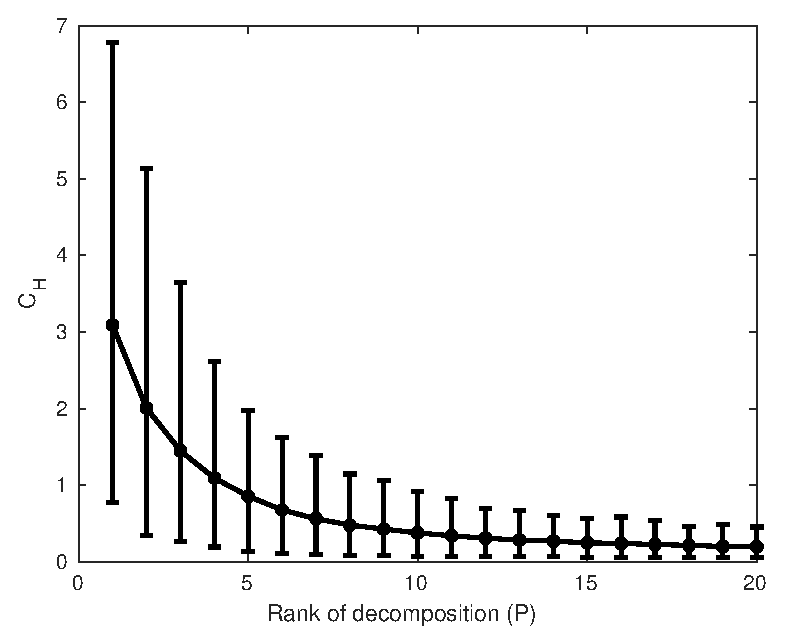
\includegraphics[width=\linewidth]{fig/RIR_NMF_approx_cost_error_plot.eps}
\caption{Effect of varying rank $P$ on the low-rank approximation for the RIR spectrogram. The deviation from the original RIR spectrogram reduces with increasing $P$. The deviation is small for $P>10$.}
\label{fig:rank_p_approximation}
\end{figure}
\iffalse
\begin{figure*}[ht]
\begin{tabular}{cccc}
\subfloat[]{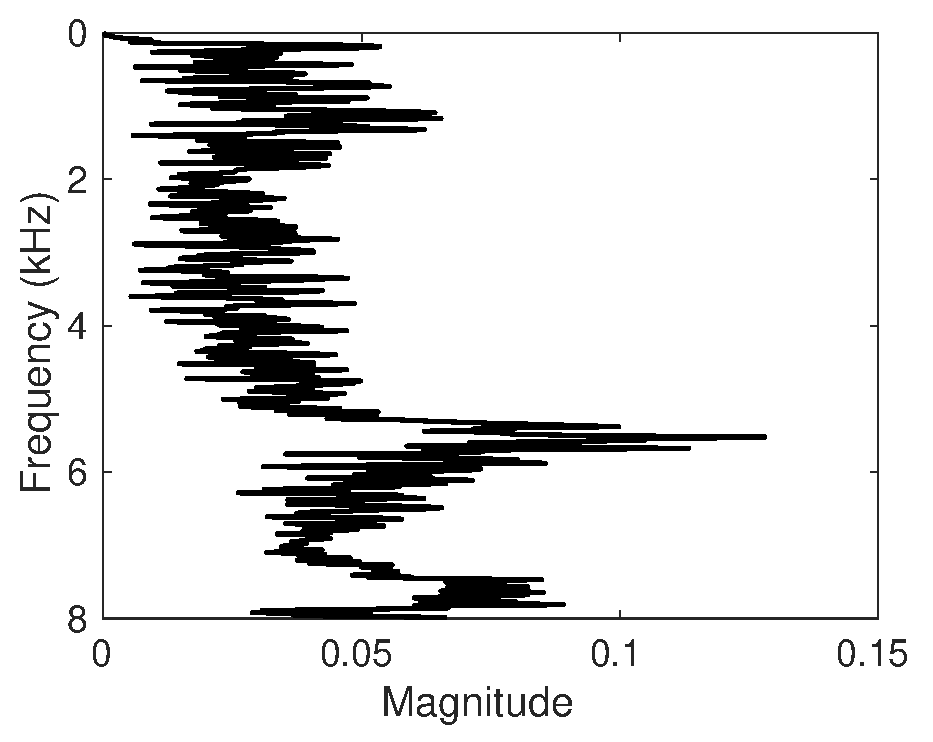
\includegraphics[width = 0.25\linewidth]{fig/RIR_env_original_RIR_cond_RIR_SimRoom3_far_AnglA_StationaryNoise_10dB.eps}} &
\subfloat[]{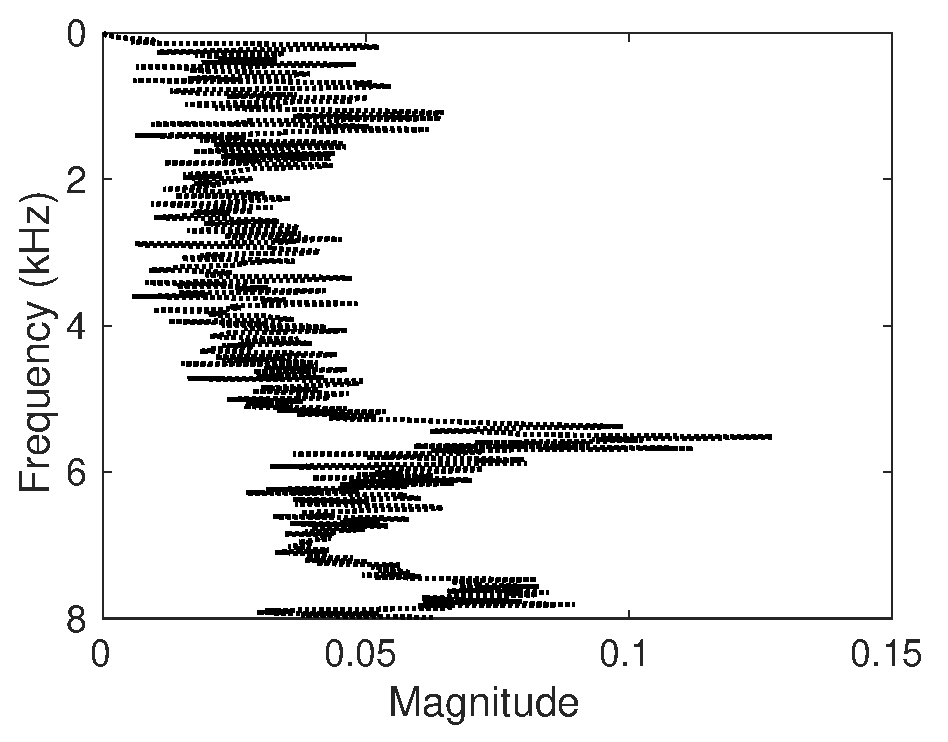
\includegraphics[width = 0.25\linewidth]{fig/RIR_env_approx_RIR_cond_RIR_SimRoom3_far_AnglA_StationaryNoise_10dB.eps}} &
\subfloat[]{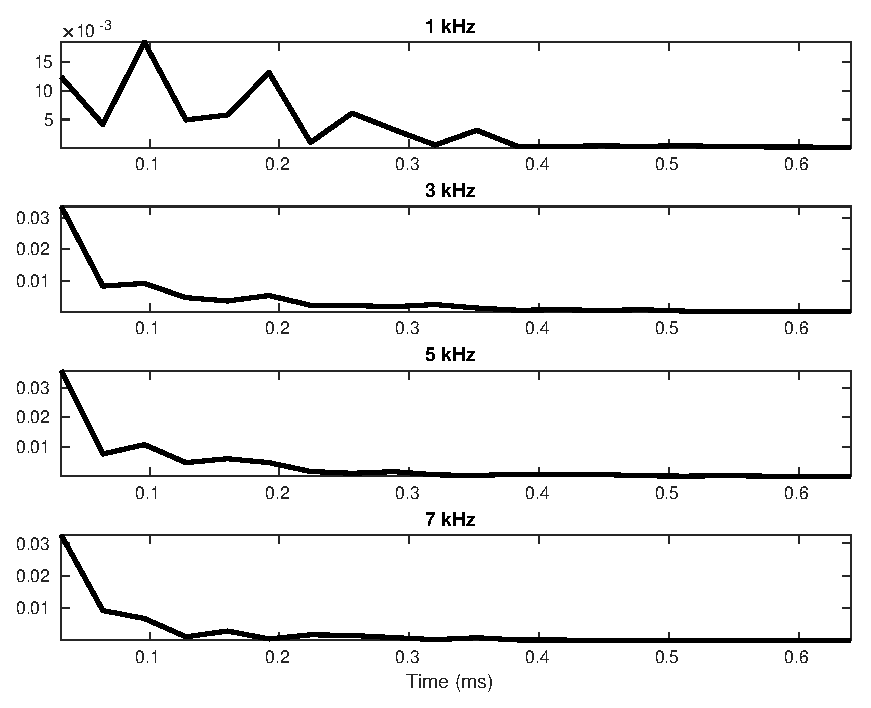
\includegraphics[width = 0.25\linewidth]{fig/RIR_tempo_original_RIR_cond_RIR_SimRoom3_far_AnglA_StationaryNoise_10dB.eps}} &
\subfloat[]{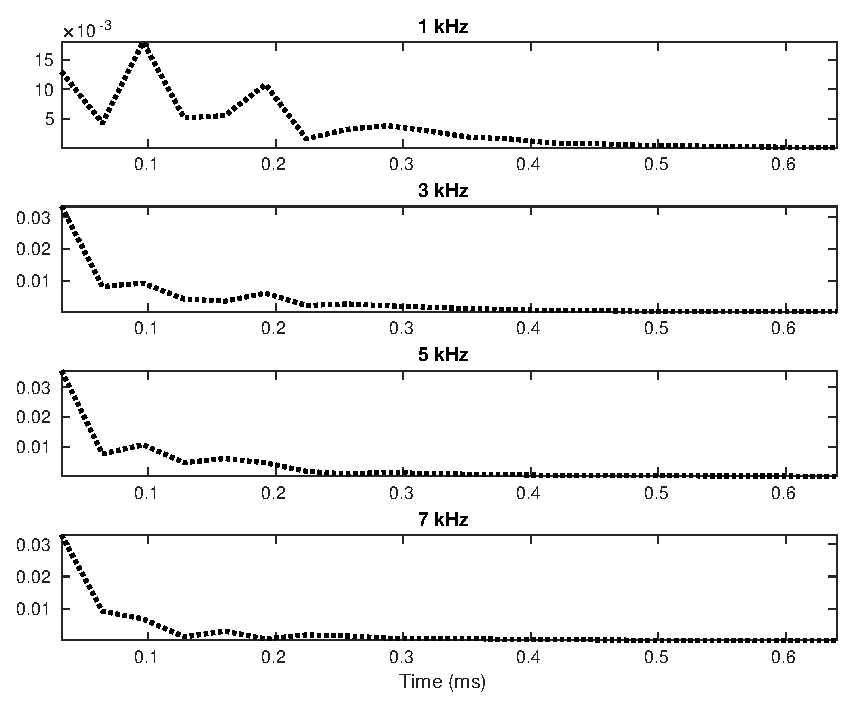
\includegraphics[width = 0.25\linewidth]{fig/RIR_tempo_approx_RIR_cond_RIR_SimRoom3_far_AnglA_StationaryNoise_10dB.eps}} \\
\end{tabular}
\caption[abc]{(a) Frequency envelope and temporal variation for different bands for the spectrogram obtained for a measured RIR from~\cite{kinoshita2016summary} having an approximate $T_{60}$ of $500$~ms and source-to-microphone distance (d) of $2$~m. (b) Frequency envelope and temporal variation obtained by a rank-$10$ NMF decomposition of the RIR. (b) is a very good approximation of (a).}
\label{fig:RIR_spectrogram}
\end{figure*}
\fi
%\iffalse
\begin{figure*}[ht]
\begin{tabular}{cc}
\subfloat[]{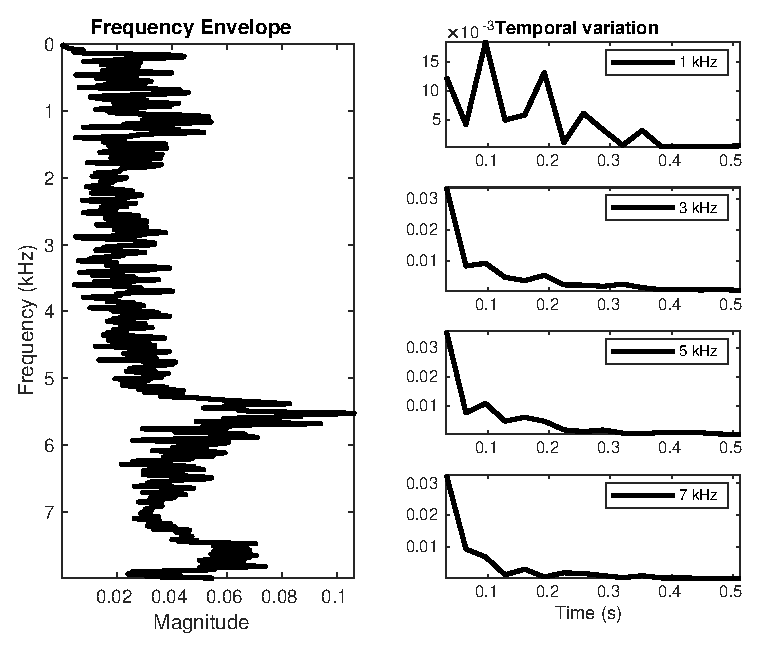
\includegraphics[width = 0.5\linewidth]{fig/RIR_NMF_far_original.eps}} &
\subfloat[]{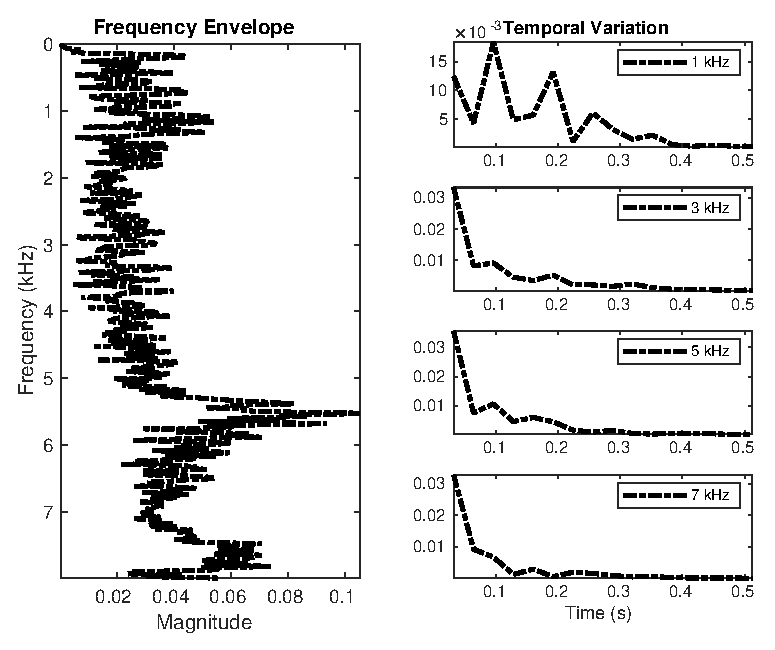
\includegraphics[width = 0.5\linewidth]{fig/RIR_NMF_far_approx.eps}}\\
\end{tabular}
\caption{(a) Frequency envelope and temporal variation obtained for a measured RIR from~\cite{kinoshita2016summary} with $T_{60}\approx 700$~ms and source-to-microphone distance $d=2$~m. (b) Frequency envelope and temporal variation obtained by a rank-$10$ NMF decomposition of the RIR. (b) is a very good approximation of (a).}
\label{fig:RIR_spectrogram}
\end{figure*}
%\fi
\iffalse
\begin{figure*}
\begin{tabular}{cc}
\subfloat[]{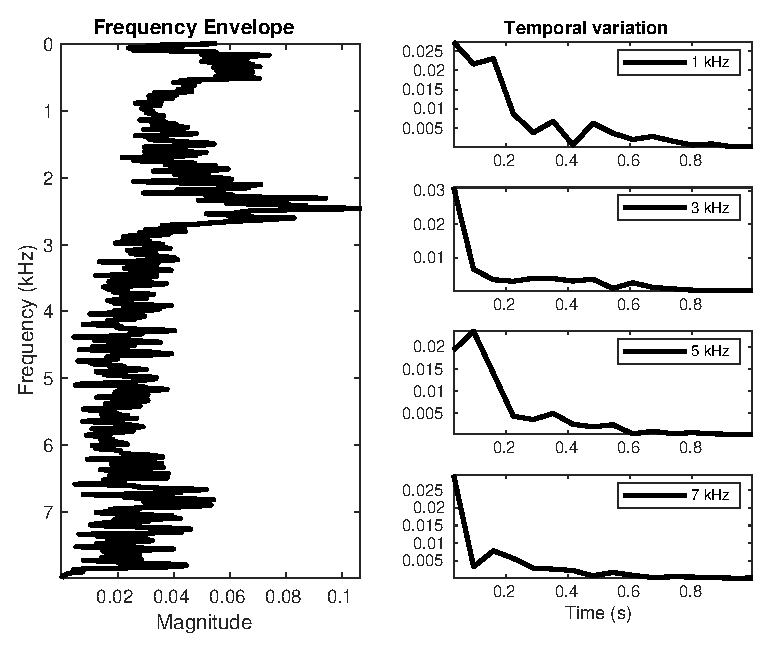
\includegraphics[width = 0.5\linewidth]{fig/RIR_NMF_near_original.eps}} &
\subfloat[]{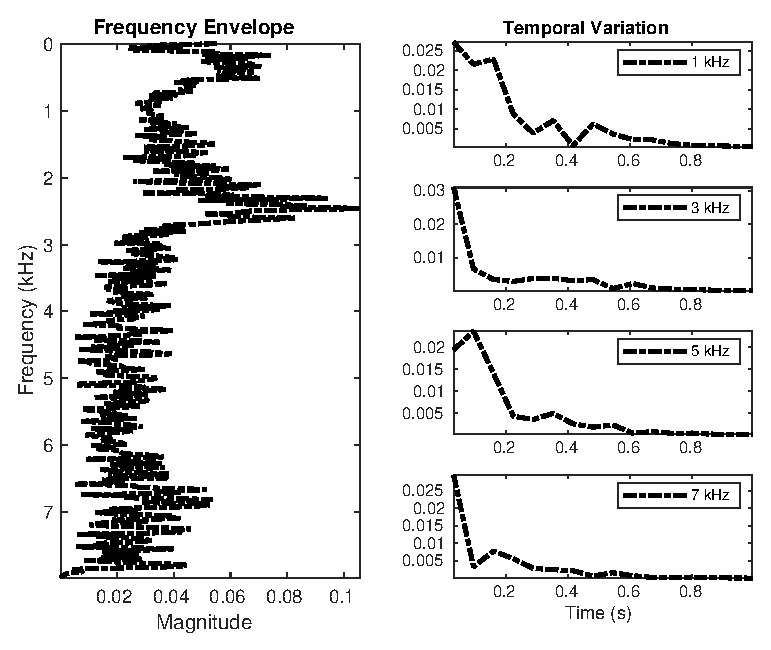
\includegraphics[width = 0.5\linewidth]{fig/RIR_NMF_near_approx.eps}}\\
\end{tabular}
\caption[abc]{(a) Frequency envelope and temporal variation for the spectrogram obtained for a measured RIR from~\cite{kinoshita2016summary} having an approximate $T_{60}$ of $500$~ms and source-to-microphone distance (d) of $0.5$~m. (b) Frequency envelope and temporal variation obtained by a rank-$10$ NMF decomposition of the RIR. (b) is a very good approximation of (a).}
%\label{fig:RIR_spectrogram}.
\label{fig:RIR_spectrogram_near}
\end{figure*}
\fi

Most of the NMF based reverberation models in literature have not considered a time-frequency model for the RIR spectrogram, though a model for speech was used. In [22], we proposed a time-frequency model for RIR spectrogram using a separability assumption. The model approximates the RIR spectrogram with a rank-$1$ NMF decomposition ($H(n, k) \approx H_1(k)H_2(n)$), where $H_1(k)$ and $H_2(n)$ represent the frequency envelope and temporal variation of RIR spectrogram, respectively. A speech enhancement algorithm was proposed using the model. It was experimentally observed that the estimated $H_1(k)$ was a good approximation to the actual frequency envelope. Further, the temporal variation $H_2(n)$ was observed to decay with $n$. The limitation of the model is it does not capture the frequency-dependent temporal variation for the RIR spectrogram. We extend the earlier model to overcome the limitation. Instead of the separability assumption used in the earlier work, we propose to use a low-rank approximation of the RIR spectrogram. The approximate RIR spectrogram is obtained using a rank-$P$ NMF decomposition. The NMF decomposition ensures that the approximated RIR spectrogram is non-negative.
%This is a requirement for using NMF based degradation model. 
The rank-$P$ NMF approximation for RIR spectrogram $\mathbf{H}$ is given by,
%Most of the NMF based reverberation models in literature have not considered a time-frequency model for the RIR spectrogram. In~\cite{mohanan201a}, we proposed a time-frequency model for RIR spectrogram using a separability assumption. The model approximates the RIR spectrogram with a rank-$1$ NMF decomposition ($H(n,k)\approx H_1(k)H_2(n)$), where $H_1(k)$ and $H_2(n)$ represent the frequency envelope and temporal variation of RIR spectrogram, respectively. A speech enhancement algorithm was proposed using the model. It was experimentally observed that the estimated $H_1(k)$ was a good approximation to the actual frequency envelope. Further, the temporal variation $H_2(n)$ was observed to decay with $n$. The limitation of the model is it cannot have frequency-dependent temporal variation for the RIR spectrogram. We extend the earlier model to overcome the limitation. Instead of the separability assumption used in the earlier work, we propose to use a low-rank approximation of the RIR spectrogram. The approximate RIR spectrogram is obtained using a rank-$P$ NMF decomposition. The NMF decomposition ensures that the approximated RIR spectrogram is non-negative. This is a requirement for using NMF based degradation model. 
%The rank-$P$ NMF approximation for RIR spectrogram $\mathbf{H}$ is represented as,
\begin{align}
\mathbf{H}&\approx\mathbf{\hat{H}}=\mathbf{H}_1\mathbf{H}_2 \nonumber \\
		  &=\underbrace{[\mathbf{H}_1^{(1)} | \mathbf{H}_1^{(2)} | ...|\mathbf{H}_1^{(P)} ]}_\textrm{$\mathbf{H}_1$} \text{ }
		  \underbrace{[\mathbf{H}_2^{(1)^T} | \mathbf{H}_2^{(2)^T} | ...|\mathbf{H}_2^{(P)^T} ]^T}_\textrm{$\mathbf{H}_2$},
\label{eq:rank-P approx}
\end{align}
where $\mathbf{H}_1^{(p)}\in \mathbb{R}_+^{K \times 1}$, and $\mathbf{H}_2^{(p)}\in \mathbb{R}_+^{1 \times L_h}$ represent the $p$-th column of $\mathbf{H}_1\in \mathbb{R}_+^{K \times P}$, and the $p$-th row of $\mathbf{H}_2\in \mathbb{R}_+^{P \times L_h}$, respectively. (\ref{eq:rank-P approx}) can also be written as,
\begin{equation}
H(k,n) \approx \sum_{p=1}^P H_1^{(p)}(k)H_2^{(p)}(n),
\label{eq:rank-P approx1}
\end{equation}
where $H_1^{(p)}(k)$ and $H_2^{(p)}(n)$ represent the $k$-th element of $\mathbf{H}^{(p)}_1$ and the $n$-th element of $\mathbf{H}^{(p)}_2$, respectively. 
The number of elements used to represent RIR spectrogram reduces from $KL_h$ to $P(K + L_h)$\footnote{The rank-$P$ used will be such that $P<L_h$ and $P << K$.}.
The elements of $\mathbf{H}_1$ and $\mathbf{H}_2$ can also be viewed in the following way. $\mathbf{H}_1^{(p)}, p \in \{1,2,...,P\}$ forms a set of $P$ frequency envelopes and $\mathbf{H}_2^{(p)}, p \in \{1,2,...,P\}$ forms the corresponding set of $P$ temporal variations for the RIR spectrogram, respectively. 

Experimentally it can be shown that the low-rank approximation $\mathbf{\hat{H}}$ is a good approximation for the original RIR spectrogram $\mathbf{H}$. RIRs available from REVERB challenge dataset~\cite{kinoshita2016summary} is used for the purpose. The RIR spectrogram is computed using a $64$~ms Hamming window with $32$~ms hop. NMF decomposition is performed on the RIR spectrogram for positive frequencies which are represented using $K=513$ and $L_h=32$.
A low-rank NMF factorization of the RIR spectrogram is obtained using the multiplicative algorithm proposed in~\cite{lee99}. We choose the generalized Kullback-Leibler (KL) divergence as the cost function. The cost function can be summarized as,
\begin{align}
&C_H = \underset{\mathbf{H}_1, \mathbf{H}_2}{\text{min}} \sum_{k,n}\text{KL} (H(k,n)|\hat{H}(k,n)), \nonumber \\
\text{where, } &\text{KL}(u|v) = u\text{log}(\dfrac{u}{v}) + v - u.
\label{eq:KLdiv}
\end{align} 
$\hat{H}(k,n)$ is the $(k,n)$-th element of the low-rank approximated RIR spectrogram $\mathbf{\hat{H}}$. $C_H$ captures the total deviation of $\hat{H}(k,n)$ from $H(k,n)$. This deviation $C_H$ depends on the rank $P$ of the decomposition. Figure~\ref{fig:rank_p_approximation} shows the mean and extreme variations in the cost function $C_H$ for different measured RIRs available in the REVERB challenge dataset~\cite{kinoshita2016summary}. It is observed that deviation $C_H$ reduces with $P$ and deviation saturates after $P = 10$ suggesting a rank-$10$ decomposition is sufficient to capture the variations in RIR. Figure~\ref{fig:RIR_spectrogram} (a) shows the frequency envelope and temporal variations obtained for a measured RIR having $T_{60}\approx 700$~ms and source-microphone distance $d=2$~m. Frequency envelope of the RIR spectrogram represents the magnitude spectrum obtained for the frame with maximum energy. Temporal variation for a particular frequency band $k=\kappa$ represents the variation of $H(\kappa,n)$ with $n$.
Figure~\ref{fig:RIR_spectrogram} (b) shows the frequency envelope and temporal variation obtained for a low-rank approximation for the RIR spectrogram. It can be observed that the approximation has captured most of the temporal and spectral variation of RIR spectrogram. A similar observation was observed for other measured RIRs.

%Figure~\ref{fig:rank_p_approximation} shows this variation for a measured RIR. It is observed that deviation reduces with $P$ and deviation saturates after $P=10$. Figure~\ref{fig:RIR_spectrogram}(b) shows the low-rank approximated spectrogram for the RIR spectrogram shown in Figure~\ref{fig:RIR_spectrogram}(a). It can be observed that the approximation has captured most of the temporal and spectral variation of RIR spectrogram.
%\begin{figure}
%\centering
%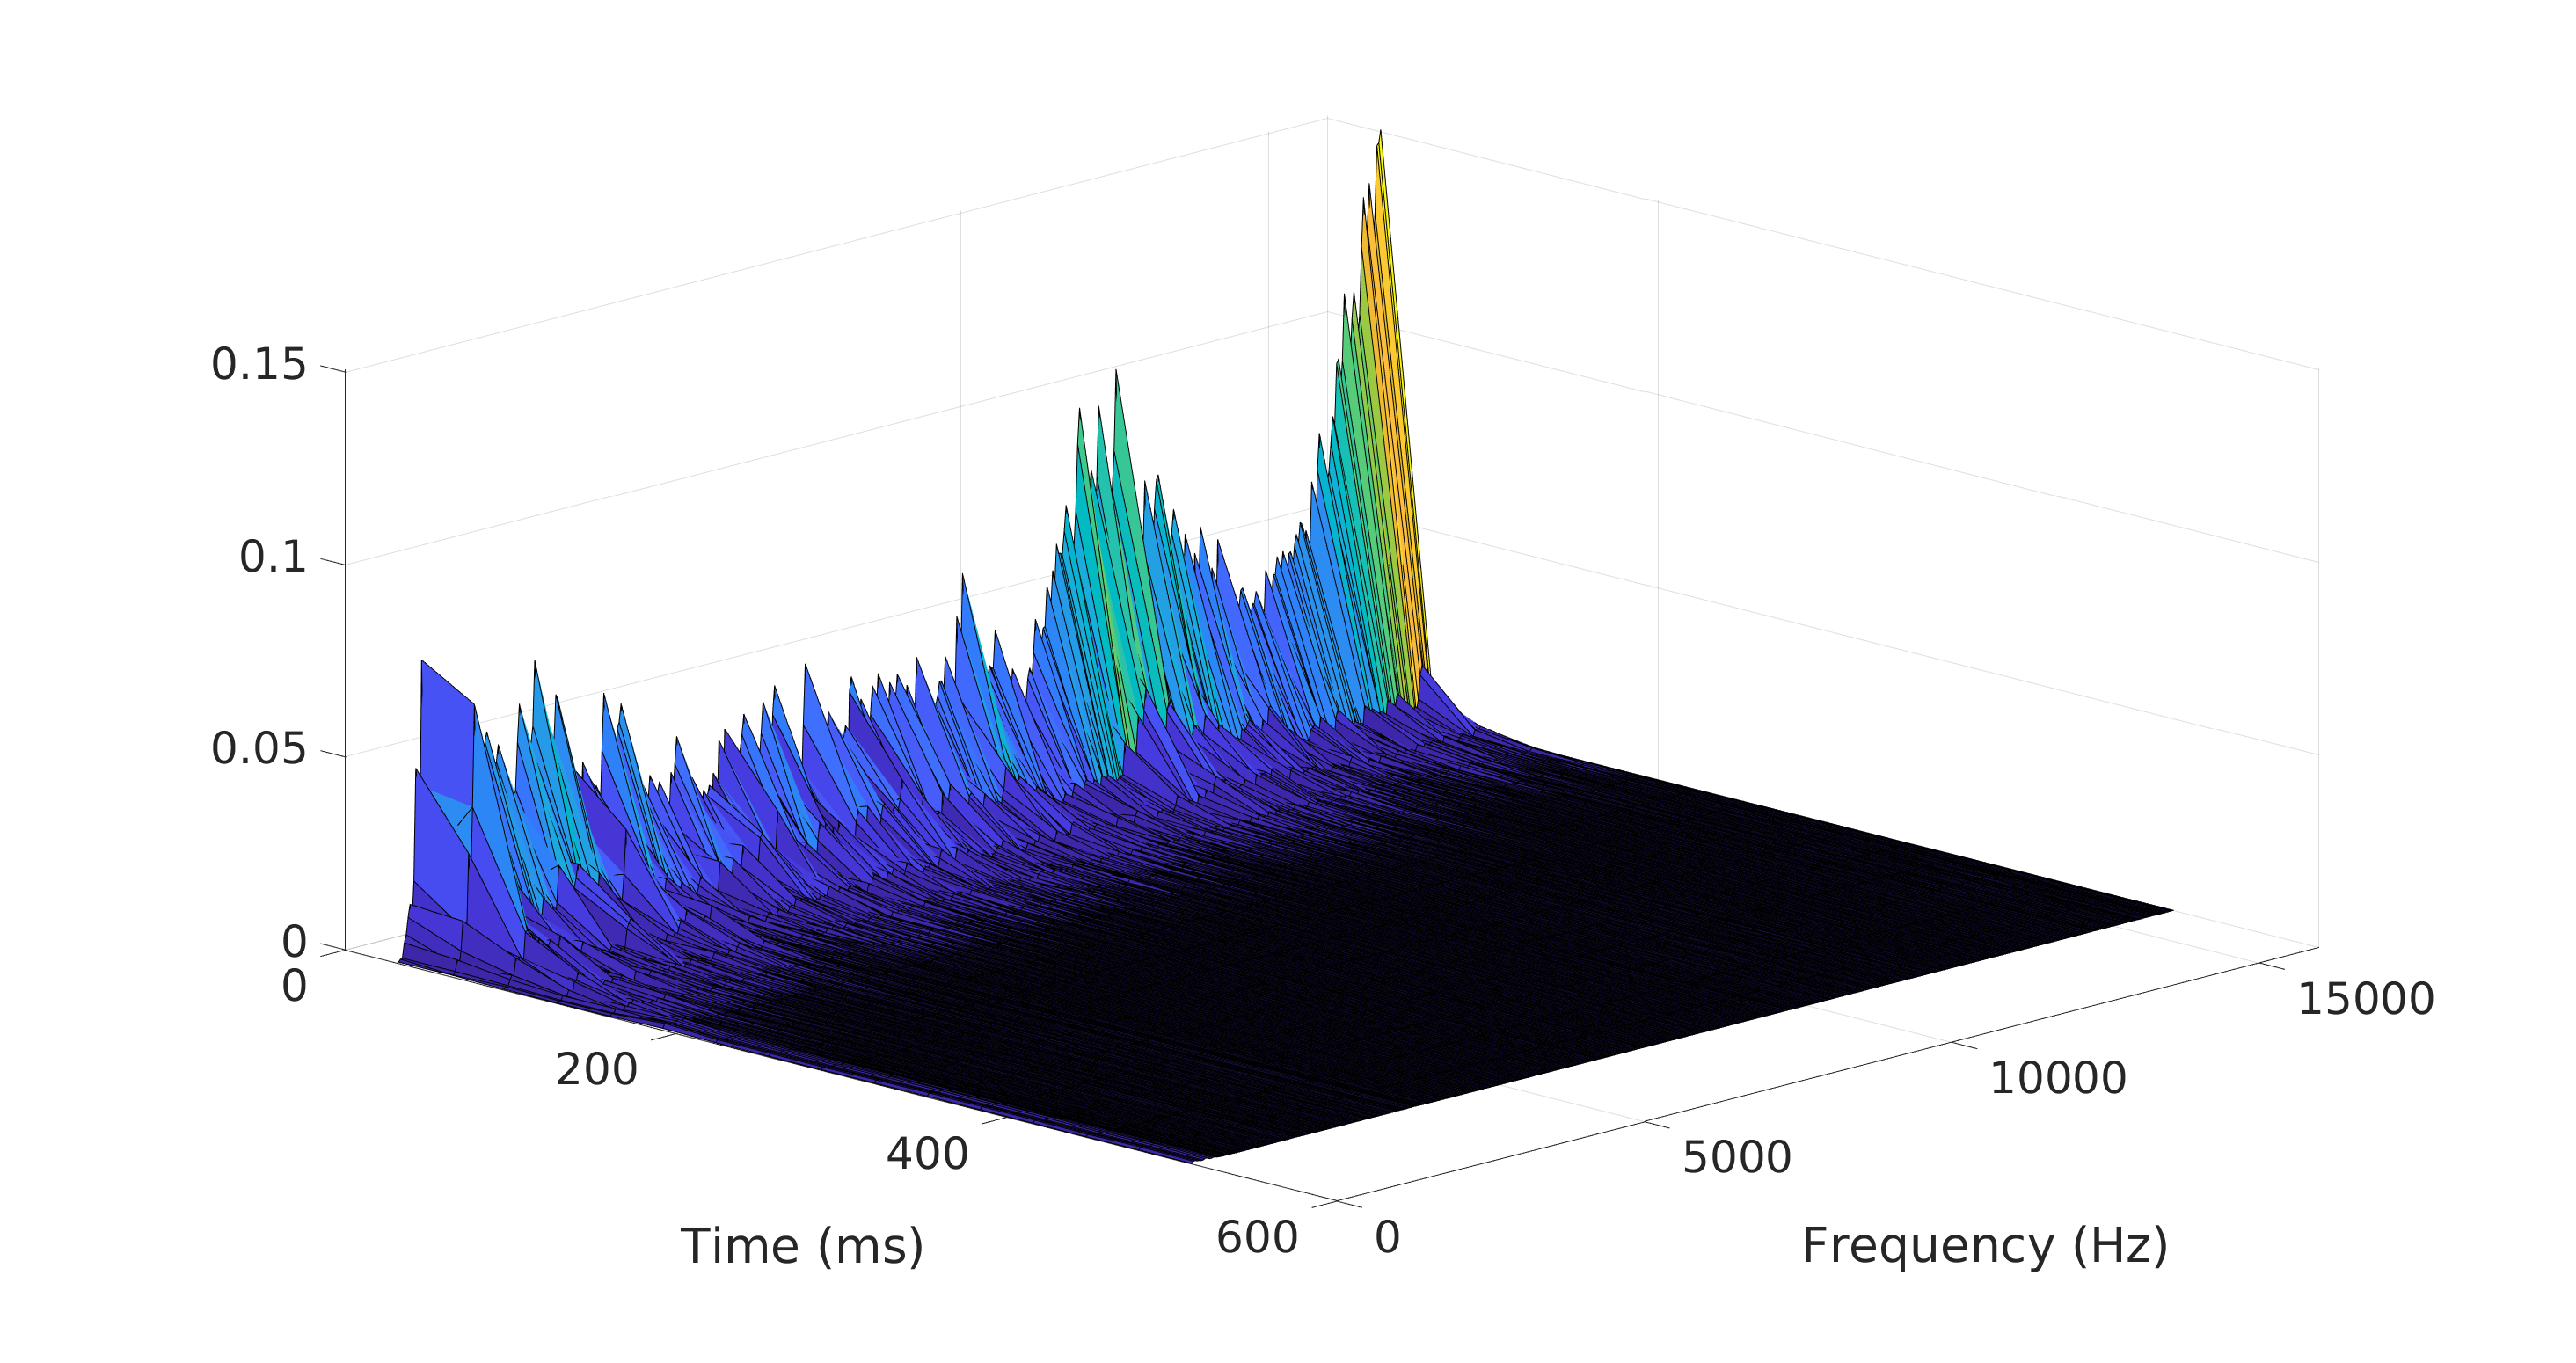
\includegraphics[width=\linewidth]{fig/RIR_approx.eps}
%\caption{The low-rank approximated RIR spectrogarm using $P=10$ for the RIR spectrogram shown in Figure~\ref{fig:RIR_spectrogram}. The original RIR spectrogram has a dimension of $513 \times 35$. The approximation is able to capture the temporal and spectral variations of the original RIR spectrogram.}
%\label{fig:RIR_approx}
%\end{figure}
%Figure~\ref{fig:RIR_spectrogram} shows the magnitude spectrogram of a measured RIR. 
%It can be observed that, the RIR spectrogram has a frequency envelope which decays with time. Also, most of the variations occur during the initial few frames after the direct path. 
\iffalse
A model for the time-frequency variation of the RIR spectrogram is discussed in \cite{wen2008blind,kuttruff2009room}. The model is based on Pollack's model for RIR. The RIR spectrogram for the model can be approximated as,
\begin{equation}
H(k,n)\approx P(k) e^{-2 \delta(k) n},
\label{eq:PollackModel}
\end{equation} 
where $P(k)$ represents the magnitude spectrum of the first frame of the RIR spectrogram ($H(k,0)$) 
%where, $P(k)$ represents the initial spectrum 
and $\delta(k)$ is related to the reverberation time ($T_{60}$) of the RIR as shown in (\ref{eq:RT60}). The $T_{60}$ (hence $\delta (k)$) changes with frequency~\cite{jeub2010we}. The variation of $T_{60}(k)$ with frequency $k$ is small for certain RIRs while for others the variation is large.  
\begin{equation}
\delta (k)= \dfrac{3\text{ln}(10)}{T_{60}(k) f_s},
\label{eq:RT60}
\end{equation}
where $f_s$ is the sampling frequency. Figure~\ref{fig:RIR_spectrogram}(a) shows the magnitude spectrogram of a measured RIR. It can be observed that the RIR spectrogram has a frequency envelope which decays with time as predicted in (\ref{eq:RT60}). The rate of decay changes with frequency as seen in the four temporal subplots in Figure~\ref{fig:RIR_spectrogram} (a) and (b). Also, most of the variations occur during the initial few frames after the direct path. The RIR spectrogram obtained based on the proposed RIR model shown in Figure~\ref{fig:RIR_spectrogram}(b) also captures these properties about RIR spectrogram. A similar behavior was observed for other RIRs and this justifies the use of the proposed RIR spectrogram model. 
\fi

\subsection{Proposed reverberation model}
This section describes the NMF model for reverberation spectrogram. Based on the low-rank approximation of the RIR spectrogram (\ref{eq:rank-P approx}), the reverb spectrogram model in (\ref{eq:deg4}) can be rewritten as,
\begin{align}
Y_R(k,n) &\approx \sum_{l=0}^{L_h-1}\sum_{p=1}^P H_1^{(p)}(k)H_2^{(p)}(l)\sum_{r=1}^R W_{\text{s}}(k,r)X_{\text{s}}(r,n-l) \nonumber \\ 
         &=\sum_{p=1}^P \sum_{r=1}^R \underbrace{W_{\text{s}}(k,r)H_1^{(p)}(k)}_\textrm{$W_R^{(p)}(k,r)$} \underbrace{ \sum_{l=0}^{L_h-1}H_2^{(p)}(l)X_{\text{s}}(r,n-l) }_\textrm{$X_R^{(p)}(r,n)$} \nonumber \\
         &= \sum_{p=1}^P \sum_{r=1}^R W_R^{(p)}(k,r)X_R^{(p)}(r,n)
\label{eq:Proposed_reverb_model}
\end{align}

Reverberation modifies the spectral and the temporal patterns of the clean speech spectrogram. In the proposed reverberation model (\ref{eq:Proposed_reverb_model}), such variations are captured by representing the reverberated speech spectrogram using NMF. The NMF model has a new set of bases $W_R^{(p)}(k,r)$ and activations $X_R^{(p)}(r,n)$. These new bases are obtained using the clean speech bases $W_{\text{s}}(k,r)$ and spectral envelopes of RIR spectrogram $H_1^{(p)}(k)$. Since the RIR spectrogram is represented using $P$ different frequency envelopes, the number of reverberated speech bases are increased by a factor of $P$. The new set of activations are obtained from clean speech activations $X_{\text{s}}(r,n)$ and temporal variation of RIR $H_2^{(p)}(n)$. The number of activations required to represent reverberated speech spectrogram also increases by a factor of $P$. This is because the RIR spectrogram contains $P$ different temporal variations. The new set of bases and activations are summarized as,
\begin{align}
W_R^{(p)}(k,r) &= W_{\text{s}}(k,r)H_1^{(p)}(k)\text{,   }p \in \{1,2,...,P\}\nonumber\\
X_R^{(p)}(r,n) &= X_{\text{s}}(r,n)*_n H_2^{(p)}(n),
\label{eq:new_model}
\end{align}
and the resulting NMF model for reverberated speech spectrogram ($\mathbf{Y}_R \approx \mathbf{W}_R\mathbf{X}_R$) is written as,
\begin{equation}
\mathbf{Y}_R \approx \underbrace{[\mathbf{W}_R^{(1)} | \mathbf{W}_R^{(2)}|...|\mathbf{W}_R^{(P)}]}_\textrm{$\mathbf{W}_R$}\ \ \underbrace{[\mathbf{X}_R^{(1)^T}|\mathbf{X}_R^{(2)^T}|...|\mathbf{X}_R^{(P)^T}]^T}_\textrm{$\mathbf{X}_R$},
\label{eq:NMF_reverb_model}
\end{equation}
%where $H_1^{(p)}(k)$ and $H_2^{(p)}(n)$ represents the $k$-th element of $\mathbf{H}^{(p)}_1$ and the $n$-th element of $\mathbf{H}^{(p)}_2$, respectively.
where $\mathbf{W}_R^{(p)} \in \mathbb{R}_+^{K \times R_s}$ and $\mathbf{X}_R^{(p)}\in \mathbb{R}_+^{R_s \times T}$ are the $p$-th block matrices of bases matrix $\mathbf{W}_R$ and activations matrix $\mathbf{X}_R$, respectively. $W_R(k,r)$ and $X_R(r,n)$ defined in (\ref{eq:new_model}) form the elements of $\mathbf{W}_R^{(p)}$ and $\mathbf{X}_R^{(p)}$, respectively. 

\subsection{Proposed joint dereverberation and denoising}
\label{sec:ProposedJointModel}
The reverberation model in~(\ref{eq:NMF_reverb_model}) can be extended to accommodate the presence of additive noise. 
The proposed approach uses an additive model to represent the degraded speech spectrogram $\mathbf{Y}$. This model is similar to the one used in~(\ref{eq:deg_model1}), where the degraded spectrogram $\mathbf{Y}$ is modeled as the sum of reverb spectrogram $\mathbf{Y}_R$ and noise spectrogram $\mathbf{Z}$. Utilizing the NMF models for noise spectrogram $\mathbf{Z}$ as in~(\ref{eq:nmf2}) and the proposed NMF model for reverberated speech spectrogram as in~(\ref{eq:NMF_reverb_model}), the degraded speech spectrogram $\mathbf{Y}$ is represented as,
\begin{align}
\mathbf{Y} & \approx \mathbf{Y}_R + \mathbf{W}_{\text{n}}\mathbf{X}_{\text{n}} = [\mathbf{W}_R| \mathbf{W}_{\text{n}}][\mathbf{X}_R^T | \mathbf{X}_{\text{n}}^T]^T. 
\label{eq:new_deg_model}
\end{align}
The bases matrix  of $\mathbf{Y}$ contains a set of bases vectors $\mathbf{W}_R$ representing reverberated speech spectrogram and another set of bases vectors $\mathbf{W}_{\text{n}}$ representing noise. Similarly, $\mathbf{X}_R$ and $\mathbf{X}_{\text{n}}$ represent the activation matrix for reverberated speech and noise spectrograms, respectively. The proposed NMF model for reverberation and noise in (\ref{eq:new_deg_model}) is easy to interpret when compared with combination of CNMF and NMF model used in (\ref{eq:deg_model2}). Further, as discussed in Section~\ref{sec:RIRconstraint} the low-rank approximation on the RIR specrogram helps in imposing better constraints on the estimated RIR spectrogram which was not possible using degradation model in (\ref{eq:deg_model2}).

\iffalse
The degraded spectrogram $\mathbf{Y}$ can be viewed as the sum of reverb spectrogram $\mathbf{Y}_R$ and noise spectrogram $\mathbf{Z}$ as in \text{CNMF2\_s}. Noise spectrogram can be approximated using a NMF model as $\mathbf{Z}\approx \mathbf{W}_n \mathbf{X}_n$, where $\mathbf{W}_n$, $\mathbf{X}_n$ represent the bases and activations of noise spectrogram, respectively. 
The degraded spectrogram $\mathbf{Y}$ can be rewritten using a NMF model as
\begin{align}
\mathbf{Y} &\approx \mathbf{Y}_R + \mathbf{Z} \approx \mathbf{Y}_R + \mathbf{W}_n\mathbf{X}_n \nonumber\\
&= [\mathbf{W}_R^{(1)} | \mathbf{W}_R^{(2)}|...|\mathbf{W}_R^{(p)}| \mathbf{W}_n][\mathbf{X}_R^{(1)^T}|\mathbf{X}_R^{(2)^T}|...|\mathbf{X}_R^{(p)^T}|\mathbf{X}_n^T]^T. 
\label{eq:new_deg_model}
\end{align}
The bases vectors of $\mathbf{Y}$ include $P$ sets of vectors to represent reverb spectrogram and a set of bases vectors to represent the noise spectrogram. Similarly, activations of degraded speech spectrogram includes $P$ sets of activations to represent reverb spectrogram and a set of activations to represent noise spectrogram. 
\fi

\section{Algorithm details}
\label{sec:cost_fn}
This section provides the algorithmic details about the proposed enhancement method. This algorithm is based on the model for reverberated and noisy speech spectrogram described in Sec~\ref{sec:ProposedJointModel}. The algorithm has a cost function associated with it that provides a measure of how well the algorithm can estimate the parameters.
An iterative approach is proposed based on the cost function to obtain an estimate for the clean speech and the RIR spectrograms.  The estimated set of parameters should ideally minimize the cost function. The first part of the section presents the proposed  enhancement algorithm. The second part of the section presents the normalization used in the algorithm.
\subsection{Joint dereverberation and denoising algorithm}
The cost function used for the proposed enhancement approach is shown in (\ref{eq:cost_enhance_rank_P}). The cost function has three terms. The  first term represents the difference between the original degraded spectrogram $\mathbf{Y}$ and the predicted degraded spectrogram $\mathbf{\tilde{Y}} = [\mathbf{W}_R | \mathbf{W}_{\text{n}}][\mathbf{X}_R^T| \mathbf{X}_{\text{n}}^T]^T$ based on generalized KL divergence. The second term is introduced to impose sparsity on estimated clean speech activation $X_{\text{s}}(r,n)$. The third term is added to impose sparsity on the noise activations $X_{\text{n}}(r,n)$. 

\begin{align}
C &= \sum_{k,n}\text{KL}(Y(k,n)|\tilde{Y}(k,n)) + \nonumber \\
& \lambda_{\text{s}} \sum_{r,n} X_{\text{s}}(r,n) + \lambda_{\text{n}} \sum_{r,n} X_{\text{n}}(r,n).
\label{eq:cost_enhance_rank_P}
\end{align}
where $\tilde{Y}(k,n)$ represents the $(k,n)$-th element of estimated degraded  spectrogram $\mathbf{\tilde{Y}}$ based on the reverberation model in (\ref{eq:new_deg_model}). The proposed cost function is similar to one used for \text{CNMF2\_s}. However, the algorithms give different solutions because $\tilde{Y}(k, n)$ in the proposed methods is estimated using a NMF model in (\ref{eq:cost_enhance_rank_P}) where as in \text{CNMF2\_s} it is obtained using a CNMF model in (\ref{eq:deg_model2}).
The multiplicative updates for clean speech and noise parameters are summarized in~(\ref{eq:update_dereverb_rank_P}).
The noise bases $W_{\text{n}}(k,r)$ and activation $X_{\text{n}}(r,n)$ are updated using standard NMF update as shown~(\ref{eq:update_enhance_rank_P}).
%The multiplicative updates obtained for the $W_s(k,r)$, $X_s(r,n)$, $H_1^{(p)}(k)$ and $H_2^{(p)}(n)$ are summarized in~(\ref{eq:update_dereverb_rank_P}).
\begin{align}
W_{\text{s}}(k,r)&\leftarrow W_{\text{s}}(k,r) \dfrac{\sum_p H_1^{(p)}(k)\sum_n \dfrac{Y(k,n)}{\tilde{Y}(k,n)}X_R^{(p)}(r,n)}{\sum_p H_1^{(p)}(k) \sum_n X_R^{(p)}(r,n)} \nonumber \\
H_1^{(p)}(k) &\leftarrow H_1^{(p)}(k)\dfrac{\sum_n\dfrac{Y(k,n)}{\tilde{Y}(k,n)}\sum_r W_{\text{s}}(k,r)X_R^{(p)}(r,n)}{\sum_n \sum_r W_{\text{s}}(k,r)X_R^{(p)}(r,n)} \nonumber \\
X_{\text{s}}(r,t) &\leftarrow X_{\text{s}}(r,t) \nonumber \\ 
         \times &\dfrac{\sum_{k,n} \dfrac{Y(k,n)}{\tilde{Y}(k,n)}  \sum_p W_R^{(p)}(k,r) H_2^{(p)}(n-t)}{\sum_{k,n}  \sum_p W_R^{(p)}(k,r) H_2^{(p)}(n-t) + \lambda_{\text{s}}} \nonumber \\
H_2^{(p)}(t) &\leftarrow H_2^{(p)}(t) \nonumber\\
\times &\dfrac{\sum_{k,n} \dfrac{Y(k,n)}{\tilde{Y}(k,n)}\sum_r W_R^{(p)}(k,r)X_{\text{s}}(r,n-t)}{\sum_{k,n} \sum_r W_R^{(p)}(k,r)X_{\text{s}}(r,n-t)}
\label{eq:update_dereverb_rank_P}
\end{align}  
%The noise bases $W_n(k,r)$ and activation $X_n(r,n)$ are updated using standard NMF update as shown~(\ref{eq:update_enhance_rank_P}).
\begin{align}
W_{\text{n}}(k,r) & \leftarrow W_{\text{n}}(k,r)\dfrac{\sum_n \dfrac{Y(k,n)}{\tilde{Y}(k,n)}X_{\text{n}}(r,n)}{\sum_n X_{\text{n}}(r,n)} \nonumber \\
X_{\text{n}}(r,n) &\leftarrow X_{\text{n}}(r,n) \dfrac{\sum_k \dfrac{Y(k,n)}{\tilde{Y}(k,n)}W_{\text{n}}(k,r)}{\sum_k W_{\text{n}}(k,r) + \lambda_{\text{n}}}
\label{eq:update_enhance_rank_P}
\end{align}
The derivations for these updates are provided in Appendix~\ref{sec:nmf_update}. The proposed NMF based joint dereverberation and denoising method will be referred to as RNMF. After the proposed NMF model converges, an estimate for the clean speech spectrogram is
obtained as $S̃(k,n)=G(k,n)Y(k,n)$. The time-varying gain function $G(k,n)$ is estimated as,
\begin{equation}
G(k,n)=\dfrac{\sum_r W_{\text{n}}(k,r)X_{\text{n}}(r,n)}{\tilde{Y}(k,n)}Y(k,n)
\label{eq:gain_function}
\end{equation}
Estimating $\tilde{S}(k,n)$ using $G(k,n)$ avoids artifacts that are introduced when $\tilde{S}(k,n)$ is estimated directly from $W_{\text{n}}(k,r)$ and $X_{\text{n}}(r,n)$~\cite{mohammadiha2016speech}. In this work, clean speech bases are assumed to be known. Depending on the way noise bases are learned there can be two different approaches - supervised approach (noise bases is also known, referred to as \text{RNMF\_s}) and semi-supervised approach (noise bases is learned from the degraded data, referred as \text{RNMF\_uk}).

\iffalse
\section{Algorithm details}
\label{sec:cost_fn}
This section provides the algorithmic details about the proposed enhancement methods. These algorithms are based on the degradation models described in Sec~\ref{sec:ProposedModel}. Iterative algorithms are proposed to obtain an estimate for the clean speech and the RIR spectrograms. Each of the algorithms has a cost function associated with it. The cost function provides a measure of how well the algorithm can estimate the parameters. The estimated set of parameters should minimize the cost function. 

\subsection{Dereverberation algorithm}
This section describes the dereverberation algorithm based on the reverberation model in (\ref{eq:Proposed_reverb_model}). The following cost function is used for the purpose. 
%The proposed approach was implemented in two stages. Such an approach will be sub-optimal as the estimate of clean activations from reverb activations is independent of estimation of other parameters in the algorithm. The two stages can be combined into a single stage approach to get better results. The stages can be combined by having additional terms in the cost function which make sure the estimated parameters are proper. The cost function used for the proposed single stage approach for reverberation using separability assumption of RIR spectrogram is shown in~(\ref{eq:cost_sep_approx_rank1}).
\begin{align}
C_R &= \sum_{k,n} \text{KL}(Y_R(k,n)|\tilde{Y}_R(k,n)) + \lambda \sum_{r,n} X_s(r,n),
\label{eq:cost_dereverb_rank_P}
\end{align}
where $\tilde{Y}_R(k,n)$ represents the estimated reverb spectrogram based on the reverberation model in (\ref{eq:Proposed_reverb_model}).  The proposed cost function is similar to one used for \text{CNMF1\_s}. However, the algorithms give different solutions because $\tilde{Y}_R(k, n)$ in the proposed methods is estimated using a NMF model in (\ref{eq:cost_dereverb_rank_P}) where as in \text{CNMF1\_s} it is obtained using a CNMF model in (\ref{eq:deg4}). The cost function has two terms. The first term represents the difference between the estimated and the actual reverberation spectrograms. The clean speech activations $X_s(k, n)$ will be spares as a few bases vectors are required to represent each frame of the clean speech spectrogram. The second term in (\ref{eq:cost_dereverb_rank_P}) is introduced to obtain a sparse solution for $X_s(k, n)$. The multiplicative updates for the cost function in (\ref{eq:cost_dereverb_rank_P}) are shown in (\ref{eq:update_dereverb_rank_P}). The detailed steps are provided in Appendix~\ref{sec:update_dereverb_1},~\ref{sec:update_dereverb_2}.

\begin{align}
W_s(k,r)&\leftarrow W_s(k,r) \dfrac{\sum_p H_1^{(p)}(k)\sum_n \dfrac{Y_R(k,n)}{\tilde{Y}_R(k,n)}X_R^{(p)}(r,n)}{\sum_p H_1^{(p)}(k) \sum_n X_R^{(p)}(r,n)} \nonumber \\
H_1^{(p)}(k) &\leftarrow H_1^{(p)}(k)\dfrac{\sum_n\dfrac{Y_R(k,n)}{\tilde{Y}_R(k,n)}\sum_r W_s(k,r)X_R^{(p)}(r,n)}{\sum_n \sum_r W_s(k,r)X_R^{(p)}(r,n)} \nonumber \\
X_s(r,t) &\leftarrow X_s(r,t) \nonumber \\ 
         \times &\dfrac{\sum_{k,n} \dfrac{Y_R(k,n)}{\tilde{Y}_R(k,n)}  \sum_p W_R^{(p)}(k,r) H_2^{(p)}(n-t)}{\sum_{k,n}  \sum_p W_R^{(p)}(k,r) H_2^{(p)}(n-t) + \lambda} \nonumber \\
H_2^{(p)}(t) &\leftarrow H_2^{(p)}(t) \nonumber\\
\times &\dfrac{\sum_{k,n} \dfrac{Y_R(k,n)}{\tilde{Y}_R(k,n)}\sum_r W_R^{(p)}(k,r)X_s(r,n-t)}{\sum_{k,n} \sum_r W_R^{(p)}(k,r)X_s(r,n-t)}
\label{eq:update_dereverb_rank_P}
\end{align}
%The proposed dereverberation method is refered to as $RNMF\-P$.
%The first term in cost function minimizes the reconstruction error. The second and third terms acts as regularizes in estimating proper estimates of the clean speech bases and activations, respectively. The parameters $\alpha$ and $\beta$ represents the relative weights given for estimated of clean speech bases and activation. These parameters are fixed by cross-validation. This method is referred to as R-NMF-$1$. Multiplicative updates can be used to simultaneously estimate the parameters. The estimated update rules are listed in~(\ref{eq:mult_update_sep_approx_rank1}). 

\subsection{Joint dereverberation and denoising}
The proposed dereverberation approach can be extended to jointly handle reverberation and noise. 
%The approach is a semi-supervised approach, i.e., the noise bases are assumed to be available. 
The cost function used for the proposed enhancement approach is shown in (\ref{eq:cost_enhance_rank_P}). The cost function has a form similar to the one used in~(\ref{eq:cost_dereverb_rank_P}). The cost function has three terms. The  first term represents the difference between the original degraded spectrogram $\mathbf{Y}$ and the predicted degraded spectrogram $\mathbf{\tilde{Y}} = [\mathbf{W}_R | \mathbf{W}_n][\mathbf{X}_R^T| \mathbf{X}_n^T]^T$ based on generalized KL divergence. The second term is introduced to impose sparsity on estimated clean speech activation $X_s(r,n)$. The third term is added to impose sparsity on the noise activations $X_n(r,n)$. 

\begin{align}
C &= \sum_{k,n}\text{KL}(Y(k,n)|\tilde{Y}(k,n)) + \nonumber \\
& \lambda_s \sum_{r,n} X_s(r,n) + \lambda_n \sum_{r,n} X_n(r,n).
\label{eq:cost_enhance_rank_P}
\end{align}
The multiplicative updates obtained for the $W_s(k,r)$, $X_s(r,n)$, $H_1^{(p)}(k)$ and $H_2^{(p)}(n)$ based on the cost function (\ref{eq:cost_enhance_rank_P}) are related to updates obtained in~(\ref{eq:update_dereverb_rank_P}). In the new updates, $Y_R(k.n)$, $\tilde{Y}_R(k,n)$ and $\lambda$ used in~(\ref{eq:update_dereverb_rank_P}) are replaced by $Y(k,n)$, $\tilde{Y}(k,n)$ and $\lambda_s$, respectively. Additionally, the noise bases $W_n(k,r)$ and activation $X_n(r,n)$ are updated using standard NMF update as shown. 
\begin{align}
W_n(k,r) & \leftarrow W_n(k,r)\dfrac{\sum_n \dfrac{Y(k,n)}{\tilde{Y}(k,n)}X_n(r,n)}{\sum_nX_n(r,n)} \nonumber \\
X_n(r,n) &\leftarrow X_n(r,n) \dfrac{\sum_k \dfrac{Y(k,n)}{\tilde{Y}(k,n)}W_n(k,r)}{\sum_k W_n(k,r) + \lambda_n}
\label{eq:update_enhance_rank_P}
\end{align}
The detailed steps are shown in Appendix~\ref{sec:update_noise}. The proposed
NMF based joint dereverberation and denoising method will be referred to as RNMF. After the proposed NMF model converges, an estimate for the clean speech spectrogram is
obtained as $S̃(k,n)=G(k,n)Y(k,n)$. The time-varying gain function $G(k,n)$ is estimated as,
\begin{equation}
G(k,n)=\dfrac{\sum_r W_s(k,r)X_s(r,n)}{\tilde{Y}(k,n)}Y(k,n)
\label{eq:gain_function}
\end{equation}
%The detailed steps are shown in Appendix~\ref{sec:update_noise}.
%The proposed NMF based joint dereverberation and denoising method will be referred to as RNMF. In this experiments, clean speech bases are assumed to be known. Depending on the way noise bases are learned there can be two different approaches - supervised approach (noise bases is also known, referred to as \text{RNMF\_s}) and semi-supervised approach (noise bases is learned from the degraded data, referred as \text{RNMF\_uk}). An estimate for the clean speech spectrogram is obtained as $\tilde{S}(k,n)=G(k,n)Y(k,n)$. The time-varying gain function $G(k,n)$ is estimated as,
Estimating $\tilde{S}(k,n)$ using $G(k,n)$ avoids artifacts that are introduced when $\tilde{S}(k,n)$ is estimated directly from $W_s(k,r)$ and $X_s(r,n)$~\cite{mohammadiha2016speech}. In this work, clean speech bases are assumed to be known. Depending on the way noise bases are learned there can be two different approaches - supervised approach (noise bases is also known, referred to as \text{RNMF\_s}) and semi-supervised approach (noise bases is learned from the degraded data, referred as \text{RNMF\_uk}).
%Estimating $\tilde{S}(k,n)$ using $G(k,n)$ avoids the occurrence of artifacts which are introduced when $\tilde{S}(k,n)$ is estimated directly from $W_s(k,r)$ and $X_s(r,n)$~\cite{mohammadiha2016speech}.
\fi
\subsection{Normalization}
\label{sec:normaization}
The normalization of the estimated parameters is critical for NMF based enhancement methods. It removes the inherent scaling ambiguity present in the cost functions. Each of the clean speech and noise bases vectors learned are normalized to have unit $\ell_2$-norm. 
In~\cite{mohammadiha2016speech}, the estimated $\mathbf{H}$ is normalized to have all-one vector for first column of $\mathbf{H}$. The estimated $\mathbf{H}_1$ and $\mathbf{H}_2$ are normalized in the same manner. The columns of $\mathbf{H}_1$ are normalized to sum to one. Each columns of $\mathbf{H}_2$ are divided element-wise with the first column of $\mathbf{H}_2$. Further, in \text{CNMF1\_s}~\cite{mohammadiha2016speech} and \text{CNMF2\_s}~\cite{baby2015coupled} the estimated RIR spectrogram is truncated so that $H(k,n) \leq H(k,n-1)$. Such a constraint on the RIR spectrogram is true only for the latter frames. Some of the initial frames (especially in far cases) can have $H(k,n) > H(k,n-1)$. So, in the proposed method, the truncation on estimated $H_2^{(p)}(n)$ is applied for $n\geq10$.
The normalization used for RNMF can be summarized as
\begin{align}
\mathbf{W}_x^{(t)} &\leftarrow \dfrac{\mathbf{W}_x^{(t)}}{|| \mathbf{W}_x^{(t)}||_2}, \text{     } x\in\{\text{s, n}\}\nonumber\\
H_1^{(p)}(k) &\leftarrow \dfrac{H_1^{(p)}(k)}{ \sum_p H^{(p)}_1(k)}, \text{   }p\in \{1,2,...,P\},\nonumber\\
H_2^{(p)}(n) &\leftarrow \dfrac{H_2^{(p)}(n)}{H^{(p)}_2(1)}, \nonumber\\
H_2^{(p)}(n) &\leftarrow \text{min}(H_2^{(p)}(n), H_2^{(p)}(n-1)), \text{ } n\geq10,
\label{eq:normalizations}
\end{align}    
where $\mathbf{W}_x^{(t)}$ represents the $t$-th column of the bases matrix $\mathbf{W}_x$.

\section{Experimental setup}
This section presents the experimental setup used for the evaluation of the proposed algorithm. The algorithm is compared with CNMF0~\cite{kameoka2009robust}, \text{CNMF1\_s}~\cite{mohammadiha2016speech} and \text{CNMF2\_s}~\cite{baby2015coupled}. The performance of the algorithms is compared based on speech enhancement results. Perceptual evaluation of speech quality (PESQ)~\cite{recommendation2001perceptual}, cepstral distance (CD)~\cite{hu2008evaluation}, speech-to-reverberation modulation energy ratio  (SRMR)~\cite{falk2010non}, and Mel-frequency cepstral coefficient distance (MFCCD)~\cite{yoshioka2009integrated} are the objective measures used for evaluation. PESQ is a measure of perceptual similarity of an enhanced speech to the target speech.
CD measure correlates well with speech distortion, overall quality, and dereverberation performance. Improvements in MFCCD is related to the ASR improvements of dereverberation algorithms. SRMR gives a measure of dereverberation performance.
Table~\ref{tab:Methods} summarizes the various enhancement methods considered in this work. The methods are distinguished based on the use of NMF models for clean speech and noise spectrograms and the way noise bases $\mathbf{W}_n$ are obtained.
\begin{table}[h]
\centering
\caption{A summary of methods compared in this work. Proposed approaches are represented in bold.} 
\begin{tabular}{|l|c|c|c|c|}
\hline
\multicolumn{1}{|c|}{\multirow{2}{*}{\textbf{Method}}} & \multicolumn{2}{c|}{\textbf{Clean speech model}} & \multicolumn{2}{c|}{\textbf{Noise model}} \\ \cline{2-5} 
\multicolumn{1}{|c|}{}                                 & \textbf{Used}       & \textbf{Pre-learned bases}       & \textbf{Used}    & \textbf{Pre-learned bases}   \\ \hline
CNMF0    & $\times$     & $\times$    & $\times$     & $\times$      \\ \hline
\text{CNMF1\_s} & $\checkmark$  & $\checkmark$ & $\times$     & $\times$      \\ \hline
\text{CNMF2\_s} & $\checkmark$  & $\checkmark$ & $\checkmark$  & $\checkmark$   \\ \hline
\textbf{RNMF\_uk} & $\checkmark$  & $\checkmark$    & $\checkmark$  & $\times$   \\ \hline
\textbf{RNFM\_s}  & $\checkmark$  & $\checkmark$ & $\checkmark$  & $\checkmark$   \\ \hline
\end{tabular}
\label{tab:Methods}
\end{table}
%Some initial results on ASR performance is also discussed.
\label{sec:experiment}
\subsection{Dataset}
The degraded data was generated using clean recordings available in the TIMIT dataset~\cite{garofolo1993timit}. The set contained $16$ different utterances selected from $16$ different speakers. This set was used to analyze the performance when using speaker-dependent (SD) and speaker-independent (SI) clean speech bases vectors.

Reverberation was simulated by convolving the clean utterances with four different measured RIRs available from REVERB challenge database~\cite{kinoshita2016summary}. The RIR $T_{60}$, source-microphone distance ($d$) and direct-to-reverberation ratios
($D_{50}$) used for the measurements are summarized in in Table~\ref{tab:RIR_cond}. $D_{50}$ gives a measure of extent of spectral coloration and reverberation tail. RIRs with $d=0.5$~m have higher $D_{50}$. Effects of spectral coloration will be dominant for these RIRs. Since the proposed approach uses a model for RIR frequency envelope, the enhancement results will be better for such RIRs.
The reverberated data is also added with stationary noise (caused mainly by air conditioning systems in a room) available from REVERB challenge~\cite{kinoshita2016summary}. The reverberated and noisy speech is obtained by adding a random segment of the noise at $10$~dB and $20$~dB signal-to-noise ratios (SNRs) to the reverberated speech. 
The performance of the algorithms is compared across eight different degradation conditions (four reverberation and two SNR conditions).  

\begin{table}[ht]
\centering
\caption{The approximate $T_{60}$, source-microphone distance ($d$) and $D_{50}$ of the measured RIRs.}
\begin{tabular}{|l|c|c|c|}
\hline
\textbf{RIR} & \textbf{$T_{60}$ (ms)} & d\textbf{ (m)} & $D_{50}$\textbf{ (\%)} \\ \hline
R2\_near     & 600                    & 0.5            & 95                \\ \hline
R2\_far      & 600                    & 2.0            & 79                \\ \hline
R3\_near     & 700                    & 0.5            & 97                \\ \hline
R3\_far      & 700                    & 2.0            & 81                \\ \hline
\end{tabular}
\label{tab:RIR_cond}
\end{table}

\subsection{Spectrogram parameters and bases creation}
The enhancements are performed on the positive half of the magnitude spectrogram of the degraded speech. 
%The spectrogram parameters are fixed as in~\cite{mohammadiha2016speech}. 
This magnitude spectrogram is obtained by performing a STFT on the degraded speech utterance using a $1024$ point ($64$~ms) Hamming window with a $512$ point ($32$~ms) hop. To include the temporal context in the speech spectrograms, frame stacking of six frames was done as suggested in~\cite{mohammadiha2016speech}. Frame stacking is done by appending the frame-shifted versions of the original spectrogram to itself. The frame stacking can be summarized as
%(\ref{eq:Frame_stacking}). 
\begin{align}
\mathbf{Y}^{stack} = [\mathbf{Y}^T| \mathbf{Y}^{\leftarrow (1)^T} | \dots |\mathbf{Y}^{\leftarrow (N-1)^T}]^T.
\label{eq:Frame_stacking}
\end{align}
\iffalse
\begin{align}
\mathbf{Y}^{stack} = \begin{bmatrix}
\mathbf{Y} \\
\mathbf{Y}^{\leftarrow (1)} \\
\vdots \\
\mathbf{Y}^{\leftarrow (N-1)}
\end{bmatrix}.
\label{eq:Frame_stacking}
\end{align}
\fi
The resulting frame has a dimension of $NK \times T$, where $N$ and $\mathbf{Y}^{stack} \in \mathbb{R}_+^{NK \times T}$ represent the number of frames stacked and the stacked degraded spectrogram, respectively. $\mathbf{Y}^{\leftarrow (N-1)}$ used in (\ref{eq:Frame_stacking}) can be obtained from $\mathbf{Y}=[\mathbf{Y}_{(1)}, \mathbf{Y}_{(2)}, ...,\mathbf{Y}_{(T)}]$ as shown in (\ref{eq:Frame_shifting}).
\begin{align}
\mathbf{Y}^{\leftarrow (N)} &= \begin{bmatrix}
\underbrace{\mathbf{Y}_{(N+1)} \text{ ... } \mathbf{Y}_{(T)}}_{T-N} & \underbrace{\mathbf{0}\text{...} \mathbf{0}}_{N}
\end{bmatrix},
\label{eq:Frame_shifting}
\end{align}
\iffalse
\begin{align}
\mathbf{Y}&=[\mathbf{Y}_{(1)}, \mathbf{Y}_{(2)}, ...,\mathbf{Y}_{(T)}] \nonumber \\
\mathbf{Y}^{\leftarrow (N)} &= \begin{bmatrix}
\underbrace{\mathbf{Y}_{(N+1)} \text{ ... } \mathbf{Y}_{(T)}}_{T-N} & \underbrace{\mathbf{0}\text{...} \mathbf{0}}_{N}
\end{bmatrix},
\label{eq:Frame_shifting}
\end{align}
\fi
where, $\mathbf{Y}_{(t)}$ and $\mathbf{0}$ represent the $t$-th column of $\mathbf{Y}$ and a zero vector of length $NK$, respectively.

A set of $100$ SD bases vectors are learned for each speaker. The bases vectors are learned from nine utterances spoken by the same speaker
%. These utterances exclude the one used for evaluation. Bases vectors are learned 
by performing a NMF decomposition on the magnitude spectrogram of these utterances. The SI bases vectors are learned from the magnitude spectrogram constructed using a subset of the train set of TIMIT. $250$ utterances spoken by different speakers are randomly selected from the train set. A set of $400$ clean speech bases vectors are learned from the magnitude spectrogram of the selected utterances. 

The noise recordings available are divided equally into train and test set. The train set is used to obtain the noise bases and test set is used to simulate degraded utterances. A NMF decomposition is performed on the magnitude spectrogram of the train set to obtain a set of noise bases vectors. A set of $100$ noise bases vectors are learned for the noise condition. This forms the noise bases matrix $\mathbf{W}_n$ used in supervised enhancement methods \text{CNMF2\_s} and \text{RNMF\_s}. Supervised enhancement methods that use SD bases will use $100$ noise bases and $100$ SD clean speech bases, whereas the SI case uses $100$ noise bases and $400$ SI clean speech bases.

\subsection{Choice of initialization and hyper-parameters}
For the proposed method RNMF, the hyper-parameters are initialized in the following manner.  Initial estimates for clean speech spectrogram $\mathbf{S}$ and RIR spectrogram $\mathbf{H}$ are obtained using (\ref{eq:deg2}). Clean speech activations $\mathbf{X}_{\text{s}}$ is obtained by performing a NMF decomposition on the estimated $\mathbf{S}$. A NMF decomposition on RIR spectrogram $\mathbf{H}$ is used to get an initial estimate for $\mathbf{H}_1$ and $\mathbf{H}_2$. The reverberated speech bases $\mathbf{W}_R$ and activations $\mathbf{X}_R$ are initialized using (\ref{eq:new_model}). For the supervised method \text{RNMF\_s}, noise activations $\mathbf{X}_{\text{n}}$ is initialized with random positive numbers. For the semi-supervised approach \text{RNMF\_uk}, an initial estimate of noise bases $\mathbf{W}_{\text{n}}$ and activations $\mathbf{X}_{\text{n}}$ are obtained using multiplicative updates shown in~(\ref{eq:update_enhance_rank_P}).

The algorithms compared in this work have cost function with terms to promote sparsity. For the reference methods CNMF0 and \text{CNMF1\_s}, the sparsity terms are fixed as in the original paper. For the reference method \text{CNMF2\_s}, sparsity terms are set as $\lambda_{\text{s}} = \lambda_{\text{n}} = 10^{-8}$. It was observed that \text{CNMF2\_s} gives better results with these regularizers. The reason for such an observation was that \text{CNMF2\_s} in~\cite{baby2015coupled} was proposed to work with exemplar bases. A large number of bases vectors are required when exemplar bases are used. However, in this work learned bases are used. So, less number of bases vectors are used. Hence, the activations were less sparse. Sparsity terms used for the proposed methods differ depending on the type of clean speech and noise bases used. \text{RNMF\_s} uses $\lambda_{\text{s}}=0.1, \lambda_{\text{n}}=10^{-8}$. Sparsity terms for \text{RNMF\_uk} is fixed as $\lambda_{\text{s}}=0.1, \lambda_{\text{n}}=10$. RIR spectrograms are represented using $L_h=20$.
The rank of the RIR spectrogram decomposition was fixed as $P = 10$ based on observations made in Figure~\ref{fig:rank_p_approximation}. 
All the enhancement algorithms run for $100$ NMF iterations. The phase spectrogram of the degraded utterance along with the enhanced magnitude spectrogram was used to obtain the corresponding enhanced time-domain signal.

\begin{figure}[h]
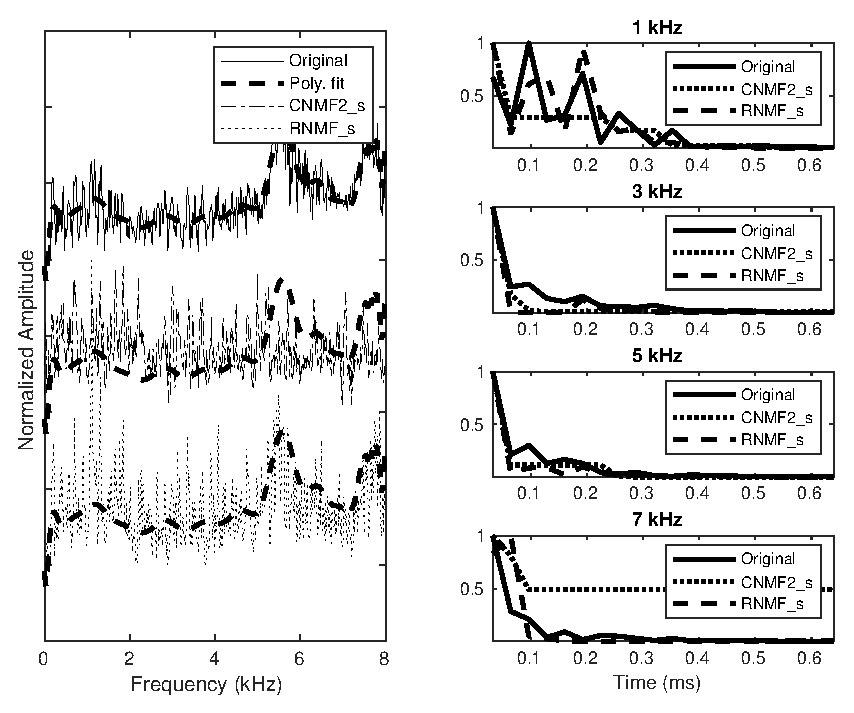
\includegraphics[width = \linewidth]{fig/RIR_comparison_SpkId_12_RIR_cond_RIR_SimRoom3_far_AnglA_StationaryNoise_10dB.eps}
\caption{Comparison of the estimated frequency envelope and temporal variation for different enhancement methods when the RIR used is \text{R3\_far}. \text{RNMF\_s} gives better RIR estimate when compared to \text{CNMF2\_s}.}
\label{fig:RIR_spectrogram_comparison}
\end{figure}
\iffalse
\begin{figure*}[h]
\begin{tabular}{cc}
\subfloat[]{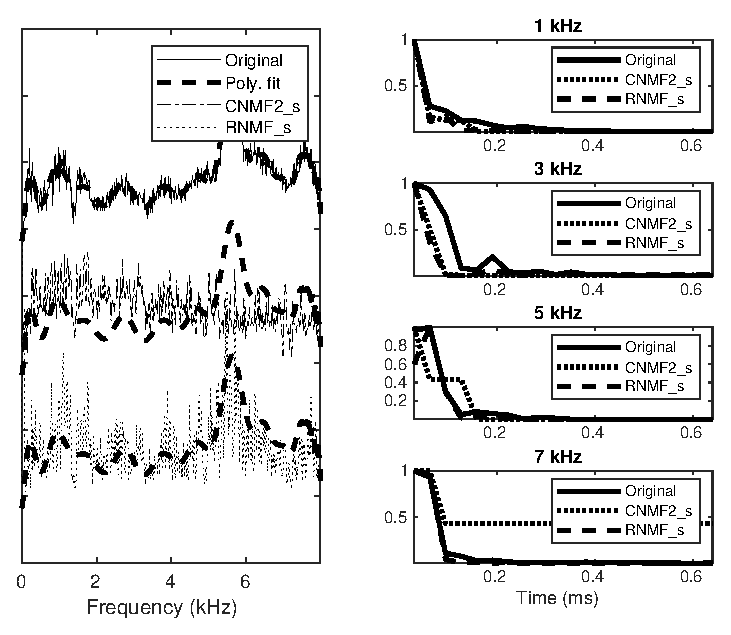
\includegraphics[width = 0.5\linewidth]{fig/RIR_comparison_SpkId_12_RIR_cond_RIR_SimRoom3_near_AnglA_StationaryNoise_10dB.eps}} &
\subfloat[]{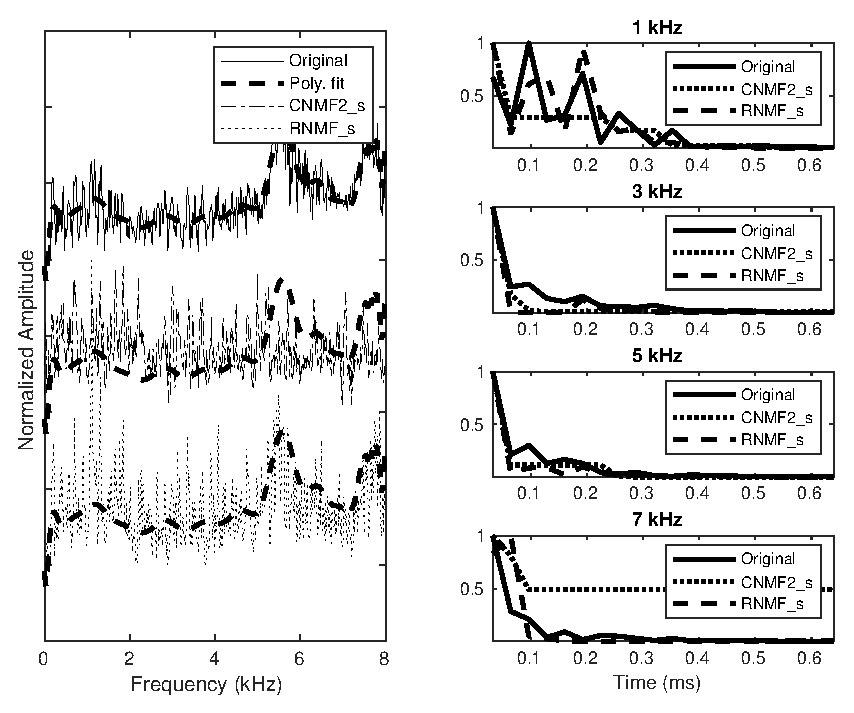
\includegraphics[width = 0.5\linewidth]{fig/RIR_comparison_SpkId_12_RIR_cond_RIR_SimRoom3_far_AnglA_StationaryNoise_10dB.eps}}\\
\end{tabular}
\caption[abc]{Frequency envelope and temporal variation for the RIR spectrogram obtained for differnt enhancement methods when (a) RIR \text{R3\_near} is used, (b) RIR \text{R3\_far} is used. RNMF methods gives better RIR estimate when compared to \text{CNMF2\_s}.}
%\label{fig:RIR_spectrogram}.
\label{fig:RIR_spectrogram_comparison}
\end{figure*}
\fi
\subsection{Results}
This section presents the performance of various enhancement methods. The proposed enhancement algorithms are compared with reference methods separately when using SD
and SI clean bases.

The performance of the various algorithms was compared for speech enhancement task. The performance was evaluated based on the relative improvements on the enhancement measures, such as PESQ~\cite{recommendation2001perceptual}, CD~\cite{hu2008evaluation},  SRMR~\cite{falk2010non}, and MFCCD~\cite{yoshioka2009integrated}. Enhanced speech is expected to have a higher PESQ and SRMR value as compared to the corresponding degraded speech. The CD and MFCCD values decrease with improving speech quality. The relative improvements in enhancement measures are represented as $\Delta$ PESQ, $\Delta$ CD, $\Delta$ SRMR, and  $\Delta$ MFCCD respectively.

The following section discusses three different experiments. The first set of experiments compares the performance of different algorithms when noise bases are unknown. The proposed algorithm \text{RNMF\_uk} is compared with CNMF0 and \text{CNMF1\_s}. Since, \text{CNMF2\_s} requires the knowledge of noise bases it is not included in this analysis. The second set of experiments compare the enhancement results when noise bases are known. \text{RNMF\_s} is compared with CNMF0, \text{CNMF1\_s} and \text{CNMF2\_s}. Finally, the estimated RIR spectrograms for different algorithms are compared.

\subsubsection{Unknown noise bases}
\label{sec:unknown_noise_cond}
Table~\ref{tab:Semi_Supervised_StationaryNoise} compares the relative improvements in objective measures obtained for different enhancement methods. The compared methods do not use any knowledge about the type of noise used. NMF speech model is used for \text{CNMF1\_s} and \text{RNMF\_uk}. The proposed method \text{RNMF\_uk} also uses a NMF model for noise. The noise bases are learned from degraded utterance. A set of $400$ bases are used to represent noise. It is observed that for the near case the proposed method \text{RNMF\_uk} consistently performs better than dereverberation only methods CNMF0 and \text{CNMF1\_s}. For the far case, all the algorithm have comparable results. Measures related to speech quality show better results, whereas measures related to ASR show slightly worse results for \text{RNMF\_uk}. The enhancement results of \text{RNMF\_uk} improves significantly when SD bases are used.
\begin{table*}[ht]
\centering
\caption{Comparison of enhancement methods in unknown noise condition.}
%\small\addtolength{\tabcolsep}{5pt}
\begin{tabular}{|l|l|l|c|c|c|c|c|c|c|c|}
\hline
\multicolumn{1}{|c|}{\multirow{2}{*}{Clean speech bases}} & \multicolumn{1}{c|}{\multirow{2}{*}{d}}                                 & \multicolumn{1}{c|}{\multirow{2}{*}{Method}} & \multicolumn{4}{c|}{SNR = 10 dB}                              & \multicolumn{4}{c|}{SNR = 20 dB}                              \\ \cline{4-11} 
\multicolumn{1}{|c|}{}                                    & \multicolumn{1}{c|}{}                                                   & \multicolumn{1}{c|}{}                        & $\Delta$ PESQ        & $\Delta$ CD          & $\Delta$ SRMR        & $\Delta$ MFCCD       & $\Delta$ PESQ        & $\Delta$ CD          & $\Delta$ SRMR        & $\Delta$ MFCCD       \\ \hline
\multirow{6}{*}{SI}                                       & \multirow{3}{*}{\begin{tabular}[c]{@{}l@{}}Near\\ (0.5 m)\end{tabular}} & CNMF0                                        & 0.13          & -0.10         & 1.47          & 0.35          & 0.21          & -0.08         & \textbf{1.45} & 0.59          \\ \cline{3-11} 
                                                          &                                                                         & CNMF1\_s                                     & 0.09          & -0.15         & 1.35          & -0.11         & 0.11          & -0.19         & 1.09          & 0.02          \\ \cline{3-11} 
                                                          &                                                                         & RNMF\_uk                                     & \textbf{0.28} & \textbf{0.10} & \textbf{1.70} & \textbf{0.66} & \textbf{0.23} & \textbf{0.16} & 1.27          & \textbf{0.60} \\ \cline{2-11} 
                                                          & \multirow{3}{*}{\begin{tabular}[c]{@{}l@{}}Far\\ (2 m)\end{tabular}}    & CNMF0                                        & 0.11          & -0.06         & 1.32          & 0.55          & 0.16          & 0.02          & 1.34          & 0.87          \\ \cline{3-11} 
                                                          &                                                                         & CNMF1\_s                                     & 0.20          & \textbf{0.19} & 1.57          & 0.93 & \textbf{0.24} & \textbf{0.43} & 1.52          & \textbf{1.46} \\ \cline{3-11} 
                                                          &                                                                         & RNMF\_uk                                     & \textbf{0.26} & 0.16          & \textbf{1.77} & \textbf{0.98} & \textbf{0.24}          & 0.35          & \textbf{2.80} & 1.21          \\ \hline
\multirow{6}{*}{SD}                                       & \multirow{3}{*}{\begin{tabular}[c]{@{}l@{}}Near\\ (0.5 m)\end{tabular}} & CNMF0                                        & 0.13          & -0.10         & 1.47          & 0.35          & 0.21          & -0.08         & \textbf{1.45} & 0.59          \\ \cline{3-11} 
                                                          &                                                                         & CNMF1\_s                                     & -0.04         & -0.05         & 1.15          & -0.41         & -0.02         & -0.11         & 0.91          & -0.33         \\ \cline{3-11} 
                                                          &                                                                         & RNMF\_uk                                     & \textbf{0.31} & \textbf{0.22} & \textbf{1.73} & \textbf{1.27} & \textbf{0.24} & \textbf{0.26} & 1.04          & \textbf{0.95} \\ \cline{2-11} 
                                                          & \multirow{3}{*}{\begin{tabular}[c]{@{}l@{}}Far\\ (2 m)\end{tabular}}    & CNMF0                                        & 0.11          & -0.06         & 1.32          & 0.55          & 0.16          & 0.02          & 1.34          & 0.87          \\ \cline{3-11} 
                                                          &                                                                         & CNMF1\_s                                     & 0.18          & 0.33          & 1.88          & 1.33          & 0.27          & 0.54          & \textbf{2.03} & 2.17          \\ \cline{3-11} 
                                                          &                                                                         & RNMF\_uk                                     & \textbf{0.36} & \textbf{0.42} & \textbf{2.08} & \textbf{1.97} & \textbf{0.39} & \textbf{0.62} & 2.02          & \textbf{2.41} \\ \hline
\end{tabular}
\label{tab:Semi_Supervised_StationaryNoise}
\end{table*}

\subsubsection{Known noise bases}
\label{sec:known_noise_cond}
Table~\ref{tab:SI_Supervised_StationaryNoise} compares the enhancement results obtained for \text{CNMF2\_s} and \text{RNMF\_s} in various degradation conditions. The enhancement methods which utilize pre-learned noise bases (\text{RNMF\_s, CNMF2\_s}) perform significantly better than dereverberation only methods (\text{CNMF0, CNMF1\_s}). This shows the merit in using the noise model. Further, the proposed method \text{RNMF\_s} performs consistently better than \text{CNMF2\_s} for the near case. The objective measures obtained \text{RNMF\_s} for far case are comparable to \text{CNMF2\_s}. Speech intelligibility measures PESQ and SRMR are better for \text{RNMF\_s}, whereas measures correlated with ASR (CD and MFCCD) are better for \text{CNMF2\_s}. Based on the enhancement results obtained for proposed enhancement methods, it can be observed that a low-rank constraint on the RIR spectrogram is helpful.

\begin{table*}[ht]
\centering
\caption{Comparison of enhancement methods that uses known noise bases.}
\begin{tabular}{|l|l|l|c|c|c|c|c|c|c|c|}
\hline
\multicolumn{1}{|c|}{\multirow{2}{*}{Clean speech bases}} & \multicolumn{1}{c|}{\multirow{2}{*}{d}}                                 & \multicolumn{1}{c|}{\multirow{2}{*}{Method}} & \multicolumn{4}{c|}{SNR = 10 dB}                              & \multicolumn{4}{c|}{SNR = 20 dB}                              \\ \cline{4-11} 
\multicolumn{1}{|c|}{}                                    & \multicolumn{1}{c|}{}                                                   & \multicolumn{1}{c|}{}                        & $\Delta$ PESQ        & $\Delta$ CD          & $\Delta$ SRMR        & $\Delta$ MFCCD       & $\Delta$ PESQ        & $\Delta$ CD          & $\Delta$ SRMR        & $\Delta$ MFCCD       \\ \hline
\multirow{4}{*}{SI}                                       & \multirow{2}{*}{\begin{tabular}[c]{@{}l@{}}Near\\ (0.5 m)\end{tabular}} & CNMF2\_s                                     & 0.18          & 0.39          & 1.08          & 1.82          & 0.13          & 0.20          & 0.51          & 1.23          \\ \cline{3-11} 
                                                          &                                                                         & RNMF\_s                                      & \textbf{0.35} & \textbf{0.64} & \textbf{2.25} & \textbf{2.63} & \textbf{0.25} & \textbf{0.54} & \textbf{1.44} & \textbf{1.69} \\ \cline{2-11} 
                                                          & \multirow{2}{*}{\begin{tabular}[c]{@{}l@{}}Far\\ (2 m)\end{tabular}}    & CNMF2\_s                                     & 0.24          & \textbf{0.58} & 1.25          & \textbf{2.31} & 0.21          & \textbf{0.59} & 0.99          & \textbf{1.97} \\ \cline{3-11} 
                                                          &                                                                         & RNMF\_s                                      & \textbf{0.27} & 0.56          & \textbf{1.91} & 2.29          & \textbf{0.26} & 0.58          & \textbf{1.97} & 1.69          \\ \hline
\multirow{4}{*}{SD}                                       & \multirow{2}{*}{\begin{tabular}[c]{@{}l@{}}Near\\ (0.5 m)\end{tabular}} & CNMF2\_s                                     & 0.09          & \textbf{0.65} & 1.15          & 3.28          & -0.09         & 0.05          & 0.30          & 1.47          \\ \cline{3-11} 
                                                          &                                                                         & RNMF\_s                                      & \textbf{0.37} & 0.64          & \textbf{2.17} & \textbf{3.80} & \textbf{0.20} & \textbf{0.26} & \textbf{1.25} & \textbf{1.68} \\ \cline{2-11} 
                                                          & \multirow{2}{*}{\begin{tabular}[c]{@{}l@{}}Far\\ (2 m)\end{tabular}}    & CNMF2\_s                                     & 0.24          & \textbf{0.93} & 1.27          & \textbf{4.27} & 0.16          & \textbf{0.62} & 0.86          & \textbf{3.10} \\ \cline{3-11} 
                                                          &                                                                         & RNMF\_s                                      & \textbf{0.43} & 0.70          & \textbf{2.75} & 4.09          & \textbf{0.38} & 0.50          & \textbf{2.69} & 2.81          \\ \hline
\end{tabular}
\label{tab:SI_Supervised_StationaryNoise}
\end{table*}

%\subsubsection{Analysis of estimate of clean speech spectrogram}
\subsubsection{Analysis of estimate of RIR}
\label{sec:RIR_estimate_comparison}
This section compares the RIR estimates obtained for the proposed method \text{RNMF\_s}
with \text{CNMF2\_s}. The comparison is done for the RIR \text{R3\_far} when noise is added at $10$~dB SNR. The normalizations used in CNMF2 s does not affect the spectral envelope of the RIR spectrogram. Hence, the obtained RIR spectrogram is assumed to be closer to the original RIR spectrogram. However, in the case of \text{RNMF\_s}, normalization on $\mathbf{H}_1$ and $\mathbf{H}_2$ removes the frequency envelope of the RIR spectrogram. So, there is a need to obtain a better RIR spectrogram estimate. This is obtained in the following manner. Once the clean speech spectrogram $S̃(k,n)$ is estimated using the time-varying gain function (\ref{eq:gain_function}), $\mathbf{X_{\text{s}}}$ is updated using a NMF decomposition on $\tilde{S̃}(k,n)$. $\mathbf{H}_1$ and $\mathbf{H}_2$ are recomputed using the proposed enhancement algorithm. While performing the re-computation, the normalization on $\mathbf{H}_1$ is avoided and the parameters $\mathbf{X}_{\text{s}}$ and $\mathbf{X}_{\text{n}}$ are kept unchanged.

Figure~\ref{fig:RIR_spectrogram_comparison} compares the RIR estimates obtained using \text{RNMF\_s} with \text{CNMF2\_s}. 
%\text{R3\_near and R3\_far} are the RIR used for the study. 
A similar observation was made for other RIRs. The plot compares the frequency envelopes and the temporal variation separately. The frequency envelope shown in the figure is normalized to have unit $\ell_2$ norm. Additionally, a $40$ degree polynomial approximation of the original frequency envelope is also shown as a dotted line. This polynomial is superimposed with the RIR estimates and is used as a reference to compare how well the spectral envelope is estimated. From the figure, it is evident that the proposed method \text{RNMF\_s} gives a better estimate for frequency envelope. The estimates of the temporal variations are normalized with the maximum value for comparison. It can be observed from the plots that the temporal variation estimate for \text{CNMF2\_s} gets saturated in many locations. This happens because of the use of truncation on the estimated RIR spectrogram (Section~\ref{sec:normaization}).   However, for the proposed method \text{RNMF\_s}, it is avoided since the truncation is done for only the later frames where it is generally true.

\subsection{Discussion}
\label{sec:discussion}
This section discusses the enhancement results. First part discusses a implicit constraint on RIR spectrogram when frame stacking is used. Next section discusses the enhancement results when different types of RIRs are used.

\subsubsection{Implicit constraint with frame stacking}
\label{sec:RIRconstraint}
The rank-$P$ for the RIR spectrogram also acts as an additional parameter in getting better clean speech spectrogram. Ideal solution for the frame stacked spectrogram of degraded speech in (\ref{eq:Frame_stacking}) is written as 

\begin{equation}
\mathbf{Y}^{stack} = \mathbf{H}^{stack}*_\text{n} \mathbf{S}^{stack} + \mathbf{Z}^{stack},
\label{eq:Frame_stacking_solution}
\end{equation}
where $\mathbf{S}^{stack}$, $\mathbf{H}^{stack}$, and $\mathbf{Z}^{stack}$ are the stacked spectrograms of clean speech $\mathbf{S}$, RIR $\mathbf{H}$ and noise spectrograms $\mathbf{Z}$, respectively. The stacked spectrograms $\mathbf{S}^{stack}$ and $\mathbf{Z}^{stack}$ are obtained in a similar manner as obtaining $\mathbf{Y}^{stack}$ from $\mathbf{Y}$ as shown in~(\ref{eq:Frame_shifting}). However, $\mathbf{H}^{stack}$ should have a structure as shown in (\ref{eq:RIR_Frame_stacking}), as the RIR spectrogram is assumed to be time-invariant. 
\begin{align}
\mathbf{H}^{stack} &= [\mathbf{H}^T|\mathbf{H}^T|...|\mathbf{H}^T]^T
\label{eq:RIR_Frame_stacking}
\end{align}
\iffalse
\begin{align}
\mathbf{H}^{stack} = \begin{bmatrix}
\mathbf{H} \\
\mathbf{H} \\
\vdots \\
\mathbf{H}
\end{bmatrix}
\label{eq:RIR_Frame_stacking}
\end{align}
\fi
The frame-shifting happening in the reverb spectrogram is due to the corresponding shift in the clean speech spectrogram.  
The frame stacked matrix, in general, can have a higher rank as compared to the original matrix. $\mathbf{Y}^{stack}$ can have a maximum rank of $N\text{ rank}(\mathbf{Y})$, $N$ represents the number of frame stacks and $\text{rank}({\mathbf{Y}})$ represents the rank of $\mathbf{Y}$. Similarly, maximum rank of $\mathbf{S}^{stack}$ and $\mathbf{Z}^{stack}$ will be $N\text{ rank}(\mathbf{S})$ and $N\text{ rank}(\mathbf{Z})$, respectively. However, $\mathbf{H}^{stack}$ will be same as $\mathbf{H}$. 
%This is because of the matrix structure of $\mathbf{H}^{stack}$ as shown in (\ref{eq:RIR_Frame_stacking}). 

The reference methods do not use any mechanism to obtain a low-rank estimate for $\mathbf{H}^{stack}$ resulting in improper estimates of $\mathbf{S}$ and $\mathbf{H}$. The proposed method implicitly imposes such a constraint. Based on the low-rank approximation of the RIR spectrogram shown in (\ref{eq:rank-P approx}), $\mathbf{H}^{stack}$ can be approximated as shown in (\ref{eq:RIR_Frame_stacking_approximation}). 
\begin{align}
\mathbf{H}^{stack} &\approx \begin{bmatrix}
\mathbf{H}_1 \mathbf{H}_2 \\
\mathbf{H}_1 \mathbf{H}_2 \\
\vdots \\
\mathbf{H}_1 \mathbf{H}_2
\end{bmatrix}
= \mathbf{H}^{stack}_1\mathbf{H}_2
\label{eq:RIR_Frame_stacking_approximation}
\end{align}
where, $\mathbf{H}^{stack}_1\in \mathbb{R}_+^{NK \times P}$ repersents the stacked version of $\mathbf{H}_1$ as shown in (\ref{eq:RIR_Frame_stacking_approximation_H1}). With low-rank approximation, $\mathbf{H}^{stack}$ is represented using a non-negative linear combination of $P$ columns of $\mathbf{H}_1^{stack}$. Hence, the rank of $\mathbf{H}^{stack}$ is $P$.
\begin{align}
\mathbf{H}^{stack}_1 &= [\mathbf{H}_1^T |\mathbf{H}_1^T | \dots | \mathbf{H}_1^T]^T 
\label{eq:RIR_Frame_stacking_approximation_H1}
\end{align}
\iffalse
\begin{align}
\mathbf{H}^{stack}_1 &= [\mathbf{H}_1^T |\mathbf{H}_1^T | \dots | \mathbf{H}_1^T]^T \nonumber \\
\text{rank}(\mathbf{H}^{stack})&=\text{rank}(\mathbf{H}_1^{stack})=P
\label{eq:RIR_Frame_stacking_approximation_H1}
\end{align}
\fi
\iffalse
\begin{align}
\mathbf{H}^{stack}_1 &= \begin{bmatrix}
\mathbf{H}_1 \\
\mathbf{H}_1 \\
\vdots \\
\mathbf{H}_1
\end{bmatrix} \nonumber \\
\text{rank}(\mathbf{H}^{stack})&=\text{rank}(\mathbf{H}_1^{stack})=P
\label{eq:RIR_Frame_stacking_approximation_H1}
\end{align}
\fi
\subsubsection{Analysis of enhancement results}
The enhancement results obtained are summarized in Tables~\ref{tab:SI_Supervised_StationaryNoise} and \ref{tab:Semi_Supervised_StationaryNoise}. It can be observed that when the source-microphone distance is small ($0.5$~m), the proposed methods consistently perform better than other methods. Also, the estimated RIR spectrogram is closer to the true RIR spectrogram. As shown in Table~\ref{tab:RIR_cond}, the $D_{50}$ is large for near cases. This indicates that the effects of spectral coloration due to RIR are significant when compared with the effects of the reverberation tail. Hence, estimating a proper RIR spectrogram resulted in better enhancement results. For RIRs in far cases ($d = 2$~m), the $D_{50}$ is relatively small, indicating that the effects of reverberation tail are significant.
Proper RIR spectrogram estimates are obtained using the proposed method. However, there are no significant improvements in enhancement results. The effects due to spectral coloration are small, so better spectral estimates do not result in any significant improvements. The temporal variations are better with the proposed method. However, the results did not change significantly, indicating that the fine details of the temporal
variations did not affect the enhancement results.

\section{Conclusion}
In this work, a novel NMF based enhancement method was proposed to jointly handle reverberation and noise. The method is based on a novel low-rank decomposition of the RIR spectrogram. The proposed semi-supervised approach showed superior enhancement results when compared with reference dereverberation methods. The proposed supervised approach gave improved enhancement results when compared to existing supervised approach. Further, the proposed algorithm was able to obtain a better estimate of RIR spectrogram. 

%\appendices
\section{NMF multiplicative update}
\label{sec:nmf_update}
%The multiplicative update rule for a variable $\mathbf{A}$ is obtained based on the the gradient $\dfrac{\partial C}{\partial \mathbf{A}}$ of the cost function $C$.
The multiplicative update rule for a variable $A$ based on the the cost function $C$ is obtained as follows $A \leftarrow A \dfrac{\dfrac{\partial C}{\partial A}^-}{\dfrac{\partial C}{\partial A}^+}$,
%\begin{align}
%A &\leftarrow A \dfrac{\dfrac{\partial C}{\partial A}^-}{\dfrac{\partial C}{\partial A}^+},
%\label{eq:multupdate}
%\end{align}
where $\dfrac{\partial C}{\partial A}^+$ and $\dfrac{\partial C}{\partial A}^-$ represents the positive and negative terms in the gradient $ \dfrac{\partial C}{\partial A}$, respectively. 
The multiplicative updates in (\ref{eq:update_dereverb_rank_P}) and (\ref{eq:update_enhance_rank_P}) dependent on the following gradients. These are computed based on the (\ref{eq:new_deg_model}).
\begin{align}
\dfrac{\partial \tilde{Y}(k,r)}{\partial W_{\text{s}}(k,r)} & =\sum_{p=1}^P H_1^{(p)}(k)X_R^{(p)}(r,n) \nonumber\\
\dfrac{\partial \tilde{Y}(k,r)}{\partial H_1^{(p)}(k)} & =\sum_r W_{\text{s}}(k,r)X_R^{(p)}(r,n) \nonumber\\
\dfrac{\partial \tilde{Y}(k,n)}{\partial X_{\text{s}}(r,t)} & =\sum_r \sum_{p=1}^P W_R^{(p)}(k,r)H_2^{(p)}(n-t) \nonumber\\
\dfrac{\partial \tilde{Y}(k,n)}{\partial H_2^{(p)}(l)} & =\sum_r \sum_{p=1}^P W_R^{(p)}(k,r)X_s(r,n-l) \nonumber\\
\dfrac{\partial \tilde{Y}(k,n)}{\partial W_{\text{n}}(r,t)} &= X_{\text{n}}(r,n) \text{,   } \dfrac{\partial \tilde{Y}(k,n)}{\partial X_{\text{n}}(r,t)} = W_{\text{n}}(k,r)  
\label{eq:intermediate_1}
\end{align}
\subsection{Update for $W_{\text{s}}(k,r)$, $H_1^{(p)}(k)$, $X_{\text{s}}(r,n)$ and $H_2^{(p)}(l)$}
\label{sec:update_dereverb_1}
%The multiplicative updates are obtained as,
\begin{align}
\dfrac{\partial C}{\partial W_{\text{s}}(k,r)} &= \sum_n \Bigg[-\dfrac{Y(k,n)}{\tilde{Y}(k,n)} \dfrac{\partial \tilde{Y}(k,r)}{\partial W_{\text{s}}(k,r)} + \dfrac{\partial \tilde{Y}(k,r)}{\partial W_{\text{s}}(k,r)} \Bigg] \nonumber \\
&= -\sum_n \dfrac{Y(k,n)}{\tilde{Y}(k,n)} \sum_{p=1}^P H_1^{(p)}(k)X_R^{(p)}(r,n)\nonumber \\ 
& + \sum_n \sum_{p=1}^P H_1^{(p)}(k)X_R^{(p)}(r,n) \nonumber \\
W_{\text{s}}(k,r) &\leftarrow W_{\text{s}}(k,r) \dfrac{\sum\limits_n \dfrac{Y(k,n)}{\tilde{Y}(k,n)}\sum\limits_{p=1}^P H_1^{(p)}(k)X_R^{(p)}(r,n)}{\sum\limits_n \sum\limits_{p=1}^P H_1^{(p)}(k)X_R^{(p)}(r,n)}
\label{eq:updateWs}
\end{align}

%The based on (\ref{eq:multupdate}) and (\ref{eq:intermediate_1}), multiplicative updates for $H_1^{(p)}$ is obtained as shown in (\ref{eq:updateH1}).
\begin{align}
\dfrac{\partial C}{\partial H_1^{(p)}(k)} &= \sum_n \Bigg[-\dfrac{Y(k,n)}{\tilde{Y}(k,n)} \dfrac{\partial \tilde{Y}(k,r)}{\partial H_1^{(p)}(k)} + \dfrac{\partial \tilde{Y}(k,r)}{\partial H_1^{(p)}(k)} \Bigg] \nonumber \\
&= -\sum_n \dfrac{Y(k,n)}{\tilde{Y}(k,n)} \sum_r W_{\text{s}}(k,r)X_R^{(p)}(r,n)\nonumber \\ 
& + \sum_n \sum_r W_{\text{s}}(k,r) X_R^{(p)}(r,n) \nonumber \\
H_1^{(p)}(k) &\leftarrow H_1^{(p)}(k) \dfrac{\sum\limits_n \dfrac{Y(k,n)}{\tilde{Y}(k,n)}\sum\limits_r W_{\text{s}}(k,r)X_R^{(p)}(r,n)}{\sum\limits_n \sum\limits_r W_{\text{s}}(k,r) X_R^{(p)}(r,n)}
\label{eq:updateH1}
\end{align}
%\subsection{Update for $X_s(r,n)$ and $H_2^{(p)}(l)$}
%\label{sec:update_dereverb_2}
%Similar to Appendix~\ref{sec:update_dereverb_1}, intermediate results required for obtaining the multiplicative update for $X_s(r,n)$ and $H_2^{(p)}(l)$ is 
%obtained as shown in (\ref{eq:intermediate_2}).
\iffalse
\begin{align}
\dfrac{\partial \tilde{Y}(k,n)}{\partial X_{\text{s}}(r,t)} & =\sum_r \sum_{p=1}^P W_R^{(p)}(k,r)H_2^{(p)}(n-t) \nonumber\\
\dfrac{\partial \tilde{Y}(k,n)}{\partial H_2^{(p)}(l)} & =\sum_r \sum_{p=1}^P W_R^{(p)}(k,r)X_{\text{s}}(r,n-l)
\label{eq:intermediate_2}
\end{align}
\fi

%The multiplicative updates are obtained as,
\begin{align}
\dfrac{\partial C}{\partial X_{\text{s}}(r,t)} &= \sum_{k,n} \Bigg[-\dfrac{Y(k,n)}{\tilde{Y}(k,n)} \dfrac{\partial \tilde{Y}(k,n)}{\partial X_{\text{s}}(r,n)} + \dfrac{\partial \tilde{Y}(k,r)}{\partial X_{\text{s}}(r,n)} \Bigg] + \lambda_{\text{s}}  \nonumber \\
&= -\sum_{k,n} \dfrac{Y(k,n)}{\tilde{Y}(k,n)} \sum_{p=1}^P W_R^{(p)}(k,r)H_2^{(p)}(n-t)\nonumber \\ 
& + \sum_{k,n} \sum_{p=1}^P W_R^{(p)}(k,r)H_2^{(p)}(n-t) + \lambda_{\text{s}}  \nonumber \\
X_{\text{s}}(r,t) &\leftarrow X_{\text{s}}(r,t) \dfrac{\sum\limits_{k,n} \dfrac{Y(k,n)}{\tilde{Y}(k,n)}\sum\limits_{p=1}^P W_R^{(p)}(k,r)H_2^{(p)}(n-t)}{\sum\limits_{k,n} \sum\limits_{p=1}^P W_R^{(p)}(k,r)H_2^{(p)}(n-t)+ \lambda_{\text{s}} }
\label{eq:updateXs}
\end{align}

%Based on (\ref{eq:multupdate}) and (\ref{eq:intermediate_2}), multiplicative updates for $H_2^{(p)}(l)$ is obtained as
\begin{align}
\dfrac{\partial C}{\partial H_2^{(p)}(l)} &= \sum_n \Bigg[-\dfrac{Y(k,n)}{\tilde{Y}(k,n)} \dfrac{\partial \tilde{Y}(k,n)}{\partial H_2^{(p)}(l)} + \dfrac{\partial \tilde{Y}(k,n)}{\partial H_2^{(p)}(l)} \Bigg] \nonumber \\
&= -\sum_k \dfrac{Y(k,n)}{\tilde{Y}(k,n)} \sum_r W_R^{(p)}(k,r)X_{\text{s}}(r,n-l)\nonumber \\ 
& + \sum_k \sum_r W_R^{(p)}(k,r) X_{\text{s}}(r,n-l) \nonumber \\
H_2^{(p)}(l) &\leftarrow H_2^{(p)}(l) \dfrac{\sum\limits_r \dfrac{Y(k,n)}{\tilde{Y}(k,n)}\sum\limits_n W_R^{(p)}(k,r)X_{\text{s}}(r,n-l)}{\sum\limits_n \sum\limits_r W_R^{(p)}(k,r) X_{\text{s}}(r,n-l)}
\label{eq:updateH2}
\end{align}

\iffalse
In Appendix~\ref{sec:update_dereverb_1} and Appendix~\ref{sec:update_dereverb_2} derive the multiplicative updates for the cost function in (\ref{eq:cost_enhance_rank_P}) were derived. A similar derivation can be done for the proposed dereverbeation problem which uses the cost function in (\ref{eq:cost_dereverb_rank_P}). For the computations $C$, $\lambda_s$, $Y(k,n)$, and $\tilde{Y}(k,n)$ used in Appendix~\ref{sec:update_dereverb_1} and Appendix~\ref{sec:update_dereverb_2} are replaced by $C_R$, $\lambda$, $Y_R(k,n)$, and $\tilde{Y}_R(k,n)$, respectively.
\fi
\subsection{Update for $W_n(k,r)$ and $X_n(r,n)$}
\label{sec:update_noise}
\iffalse
The intermediate results needed for the estimation of $W_n(k,r)$ and $X_n(r,n)$ are obtained as,
\begin{align}
\dfrac{\partial \tilde{Y}(k,n)}{\partial X_{\text{n}}(r,t)} = W_{\text{n}}(k,r) 
\label{eq:intermediate_3}
\end{align}
\fi
%Based on (\ref{eq:multupdate}) and (\ref{eq:intermediate_3}), multiplicative updates for $X_n(r,n)$ is obtained as shown next.
\begin{align}
\dfrac{\partial C}{\partial W_{\text{n}}(k,r)} &= \sum_n \Bigg[-\dfrac{Y(k,n)}{\tilde{Y}(k,n)} \dfrac{\partial \tilde{Y}(k,n)}{\partial W_{\text{n}}(k,r)} + \dfrac{\partial \tilde{Y}(k,n)}{\partial W_{\text{n}}(k,r)} \Bigg]  \nonumber \\
&= -\sum_k \dfrac{Y(k,n)}{\tilde{Y}(k,n)} X_{\text{n}}(r,n) + \sum_k X_{\text{n}}(r,n) \nonumber \\ 
W_{\text{n}}(r,n) &\leftarrow W_{\text{n}}(r,n) \dfrac{\sum\limits_n \dfrac{Y(k,n)}{\tilde{Y}(k,n)} X_{\text{n}}(r,n)}{\sum\limits_n X_{\text{n}}(r,n)}
\label{eq:updateWn}
\end{align}

\begin{align}
\dfrac{\partial C}{\partial X_n(r,t)} &= \sum_k \Bigg[-\dfrac{Y(k,n)}{\tilde{Y}(k,n)} \dfrac{\partial \tilde{Y}(k,n)}{\partial X_n(r,t)} + \dfrac{\partial \tilde{Y}(k,n)}{\partial X_n(r,t)} \Bigg] + \lambda_n \nonumber \\
&= -\sum_k \dfrac{Y(k,n)}{\tilde{Y}(k,n)} W_n(k,r) + \sum_k W_n(k,r) + \lambda_n \nonumber \\ 
X_n(k,r) &\leftarrow X_n(k,r) \dfrac{\sum_k \dfrac{Y(k,n)}{\tilde{Y}(k,n)} W_n(k,r)}{\sum_k W_n(k,r) + \lambda_n}
\label{eq:updateXn}
\end{align}

\iffalse
\section{Spectrogram comparison}
Figure~\ref{fig:Spectrogram_reverb_with_SD_bases} and Figure~\ref{fig:Spectrogram_reverb_with_SI_bases} compares the estimated reverb spectrogram using various reverberation models with the actual reverberation spectrogram when SD and SI clean speech bases are used, respectively. The compared algorithms are CNMF0, \text{CNMF1\_s} and RNMF. It can be observed that the models are a smoother version of the original reverb spectrogram. \text{CNMF\_s} and RNMF models give more smoother version of reverb spectrogram when compared with RNMF. The spectrogram plots of RNMF and \text{CNMF1\_s} are mostly same.
\begin{figure*}
\begin{tabular}{cc}
\subfloat[]{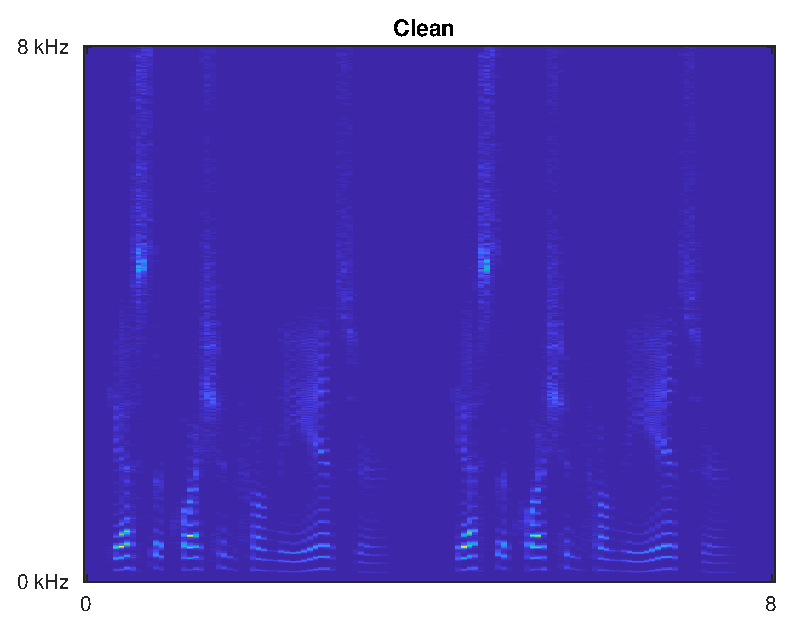
\includegraphics[width = 0.5\linewidth, height = 4cm]{fig/STFT/Sample_mjar0_clean.eps}} &
\subfloat[]{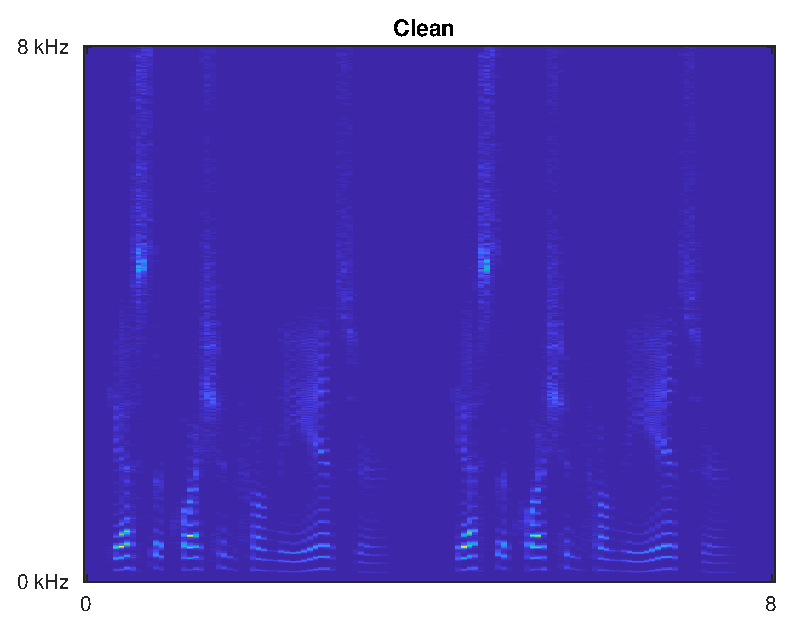
\includegraphics[width = 0.5\linewidth, height = 4cm]{fig/STFT/Sample_mjar0_clean.eps}}\\
\subfloat[]{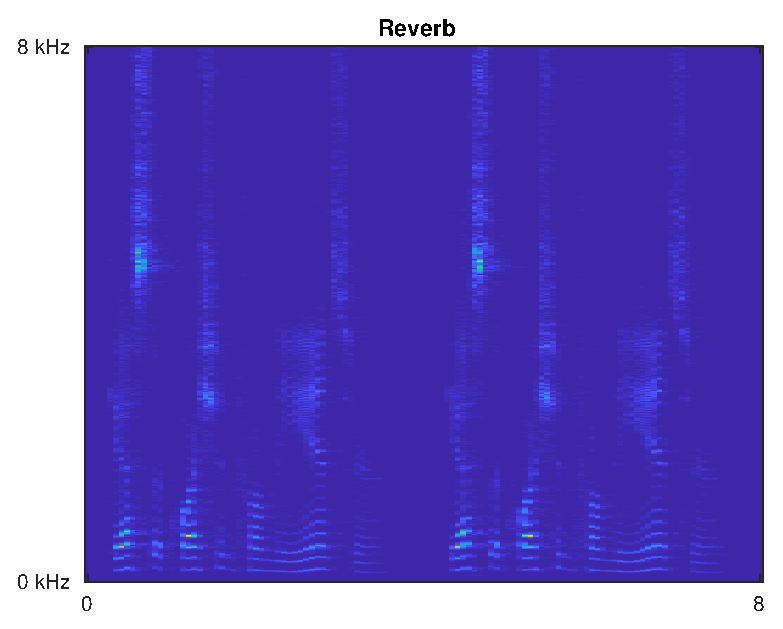
\includegraphics[width = 0.5\linewidth, height = 4cm]{fig/STFT/Sample_mjar0_reverb_RIR_SimRoom2_near_AnglA.eps}}&
\subfloat[]{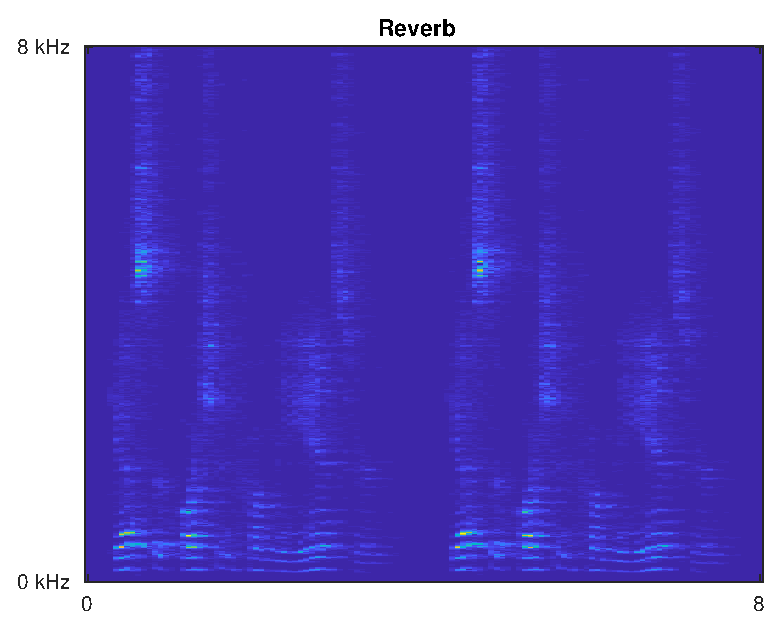
\includegraphics[width = 0.5\linewidth, height = 4cm]{fig/STFT/Sample_mjar0_reverb_RIR_SimRoom2_far_AnglA.eps}}\\
\subfloat[]{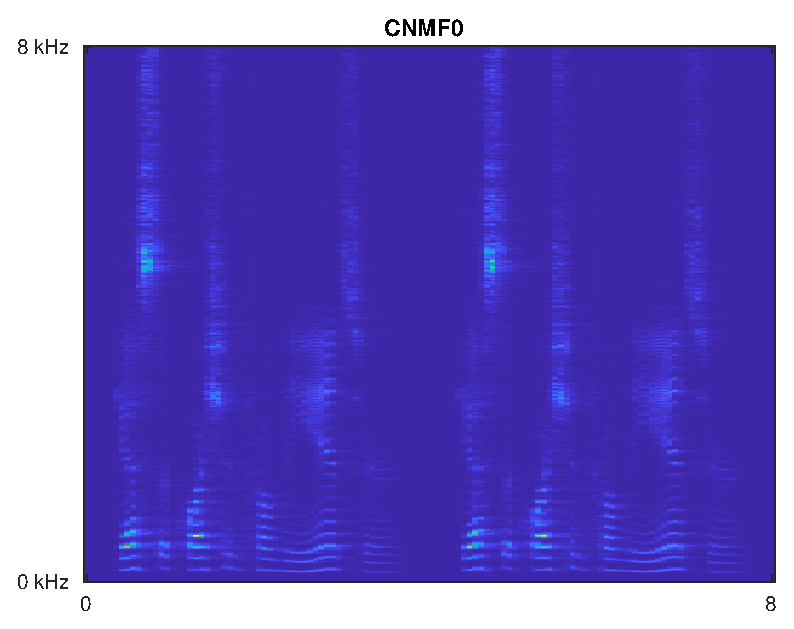
\includegraphics[width = 0.5\linewidth, height = 4cm]{fig/STFT/Sample_mjar0_CNMF0_RIR_SimRoom2_near_AnglA.eps}} &
\subfloat[]{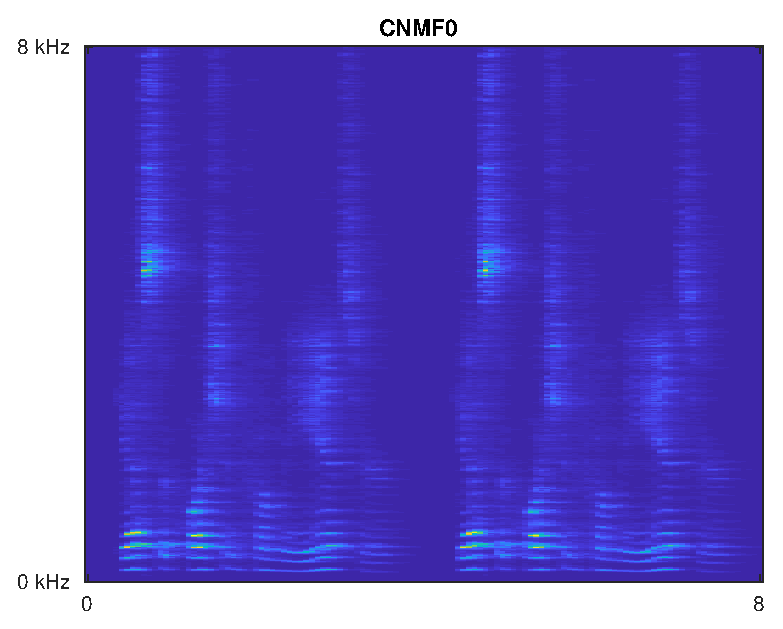
\includegraphics[width = 0.5\linewidth, height = 4cm]{fig/STFT/Sample_mjar0_CNMF0_RIR_SimRoom2_far_AnglA.eps}} \\
\subfloat[]{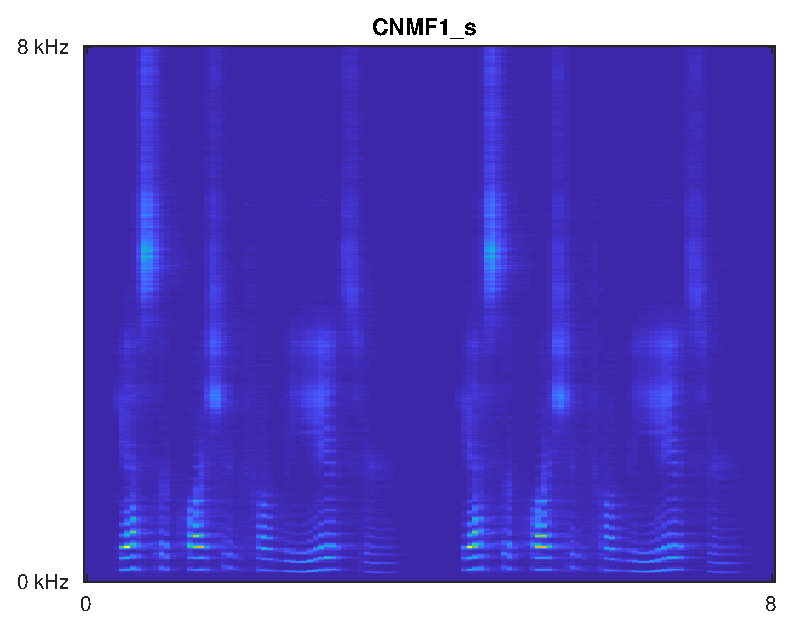
\includegraphics[width = 0.5\linewidth, height = 4cm]{fig/STFT/Sample_mjar0_SD_CNMF1_s_RIR_SimRoom2_near_AnglA.eps}}&
\subfloat[]{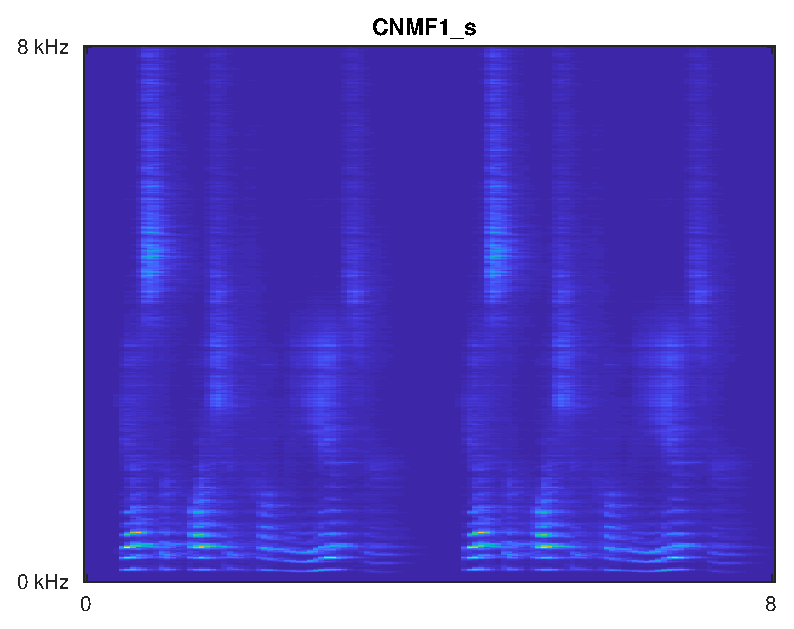
\includegraphics[width = 0.5\linewidth, height = 4cm]{fig/STFT/Sample_mjar0_SD_CNMF1_s_RIR_SimRoom2_far_AnglA.eps}}\\
\subfloat[]{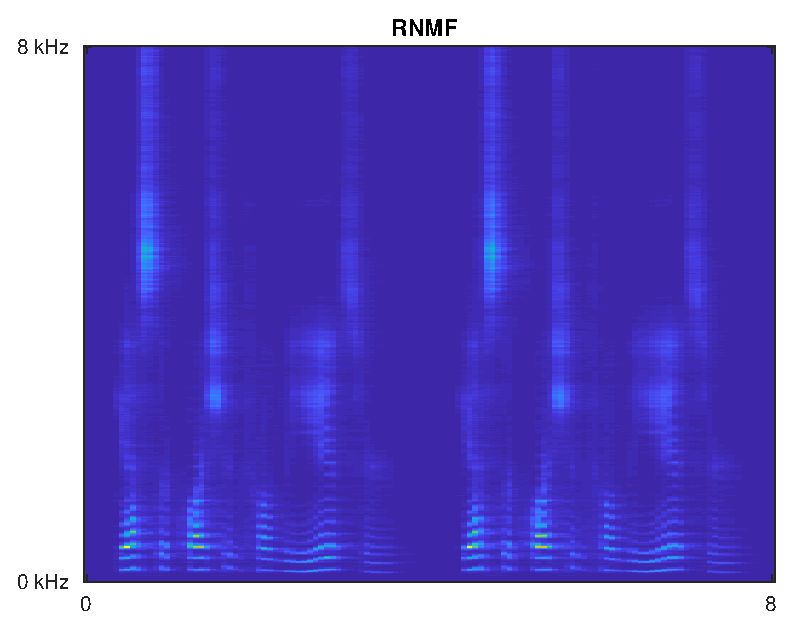
\includegraphics[width = 0.5\linewidth, height = 4cm]{fig/STFT/Sample_mjar0_SD_RNMF_RIR_SimRoom2_near_AnglA.eps}}&
\subfloat[]{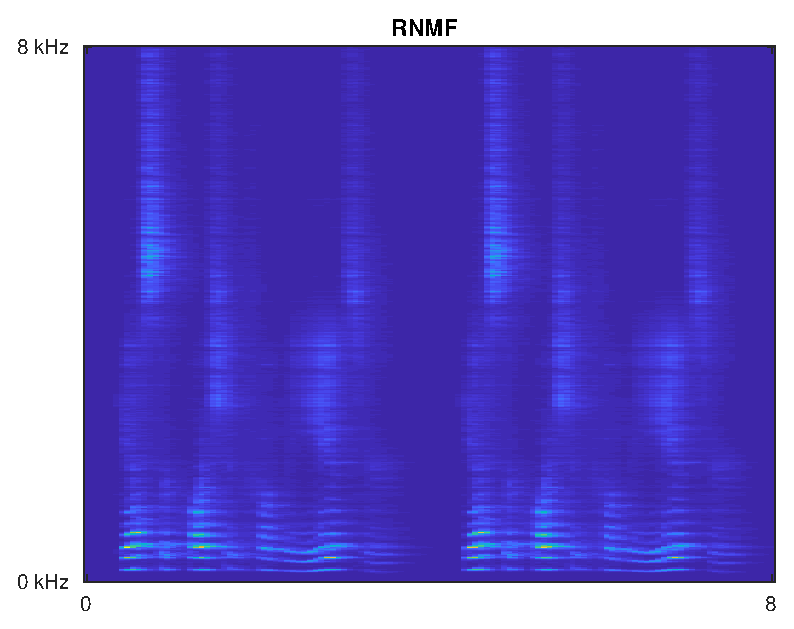
\includegraphics[width = 0.5\linewidth, height = 4cm]{fig/STFT/Sample_mjar0_SD_RNMF_RIR_SimRoom2_far_AnglA.eps}}\\
\end{tabular}
\caption[abc]{Comparison of reverb spectrogram estimated using various reverberation model when SD clean speech bases are used. Models are a smoother version of original spectrogram. The modeling error for all algorithms are small for near case. RNMF is more smoother than CNMF0. Spectrogram estimated using RNMF is mostly same as done by \text{CNMF1\_s}. }
\label{fig:Spectrogram_reverb_with_SD_bases}
\end{figure*}

\begin{figure*}
\begin{tabular}{cc}
\subfloat[]{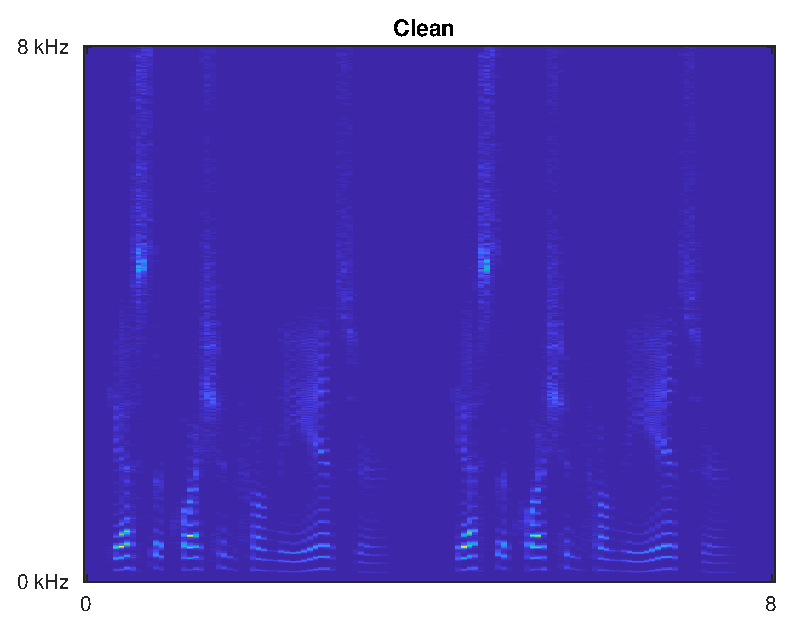
\includegraphics[width = 0.5\linewidth, height = 4cm]{fig/STFT/Sample_mjar0_clean.eps}} &
\subfloat[]{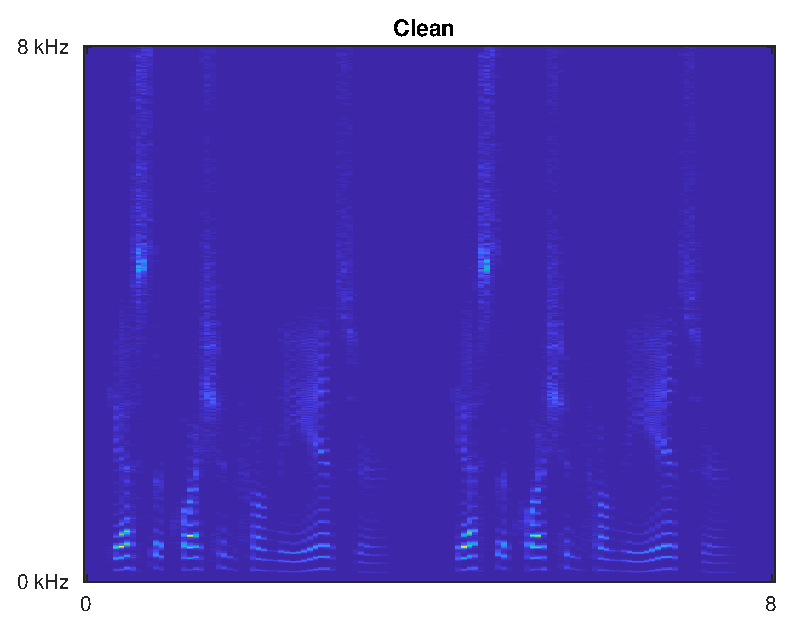
\includegraphics[width = 0.5\linewidth, height = 4cm]{fig/STFT/Sample_mjar0_clean.eps}}\\
\subfloat[]{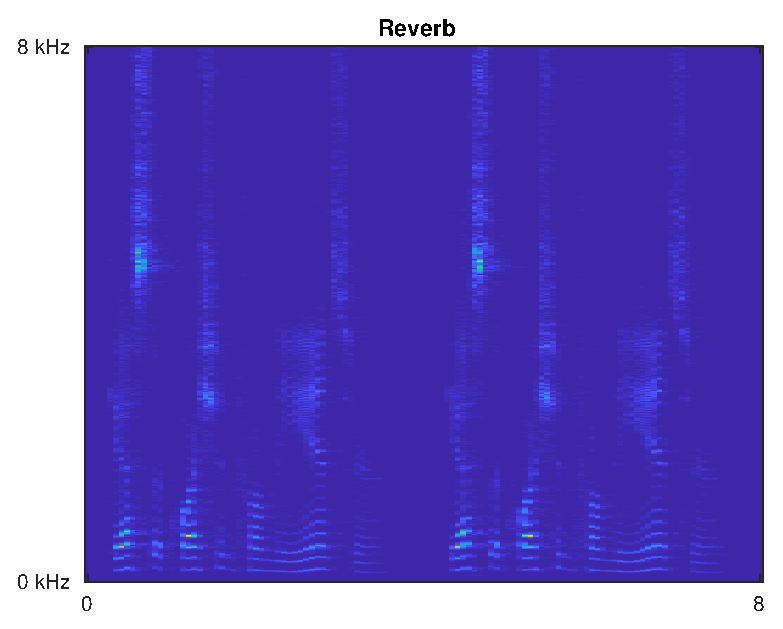
\includegraphics[width = 0.5\linewidth, height = 4cm]{fig/STFT/Sample_mjar0_reverb_RIR_SimRoom2_near_AnglA.eps}}&
\subfloat[]{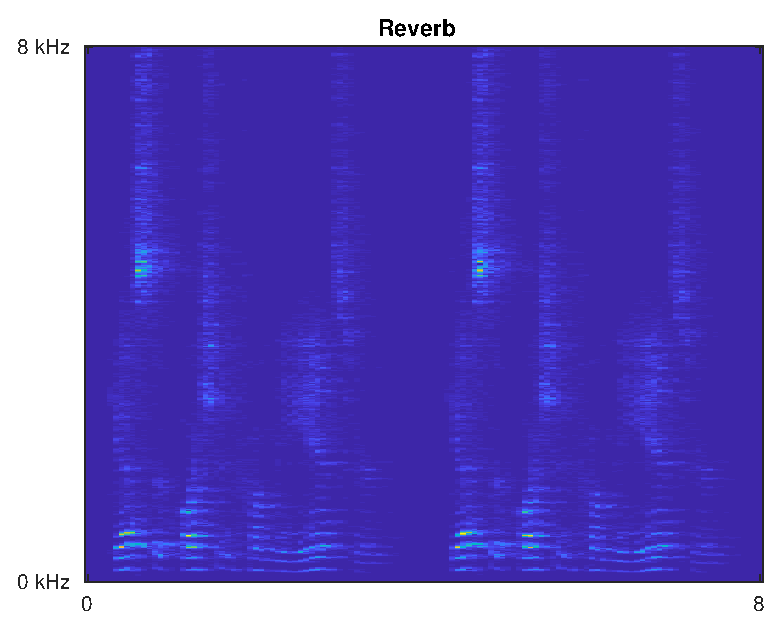
\includegraphics[width = 0.5\linewidth, height = 4cm]{fig/STFT/Sample_mjar0_reverb_RIR_SimRoom2_far_AnglA.eps}}\\
\subfloat[]{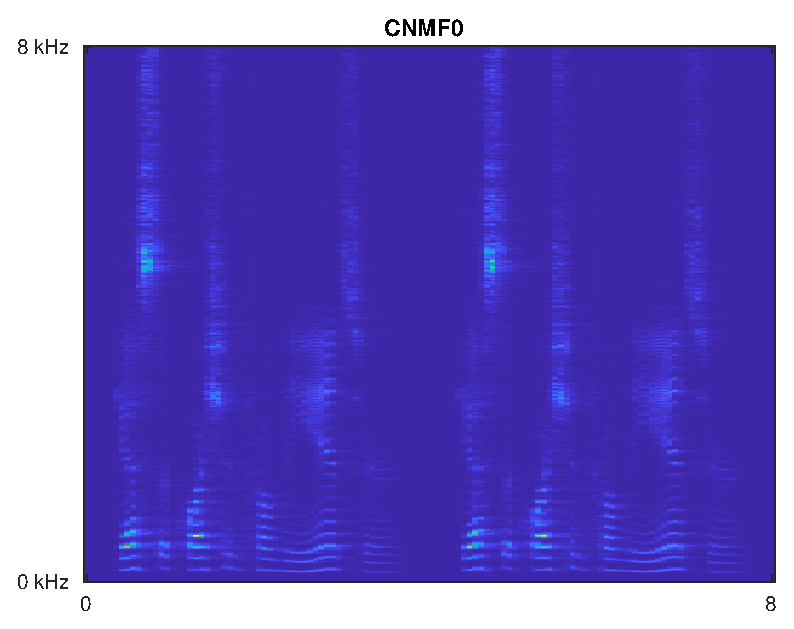
\includegraphics[width = 0.5\linewidth, height = 4cm]{fig/STFT/Sample_mjar0_CNMF0_RIR_SimRoom2_near_AnglA.eps}} &
\subfloat[]{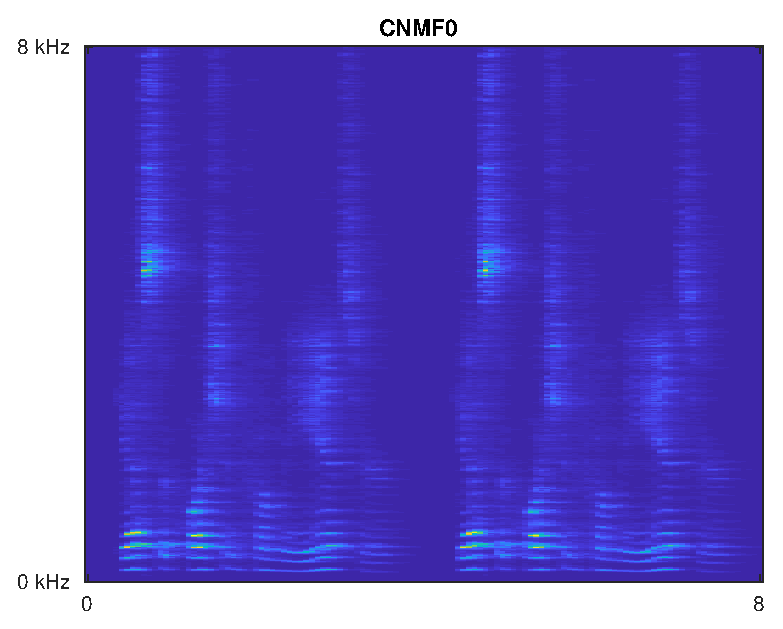
\includegraphics[width = 0.5\linewidth, height = 4cm]{fig/STFT/Sample_mjar0_CNMF0_RIR_SimRoom2_far_AnglA.eps}} \\
\subfloat[]{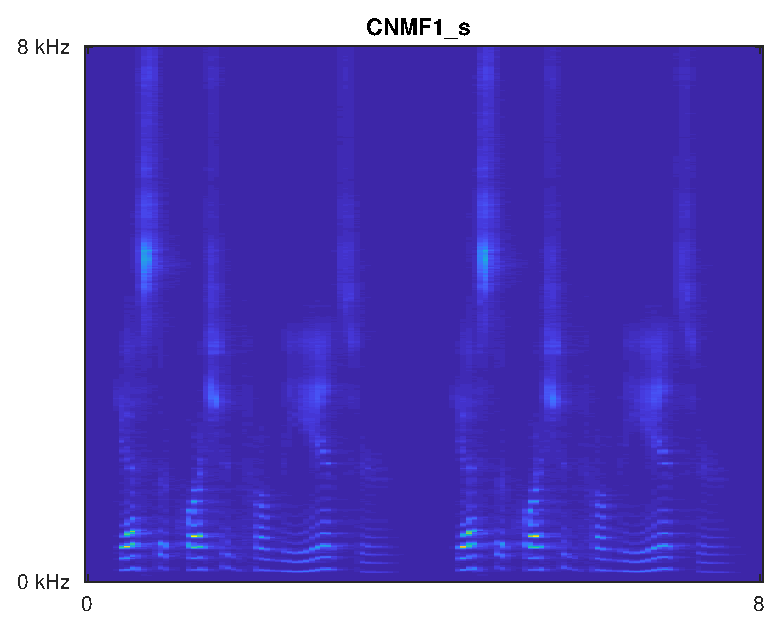
\includegraphics[width = 0.5\linewidth, height = 4cm]{fig/STFT/Sample_mjar0_SI_CNMF1_s_RIR_SimRoom2_near_AnglA.eps}}&
\subfloat[]{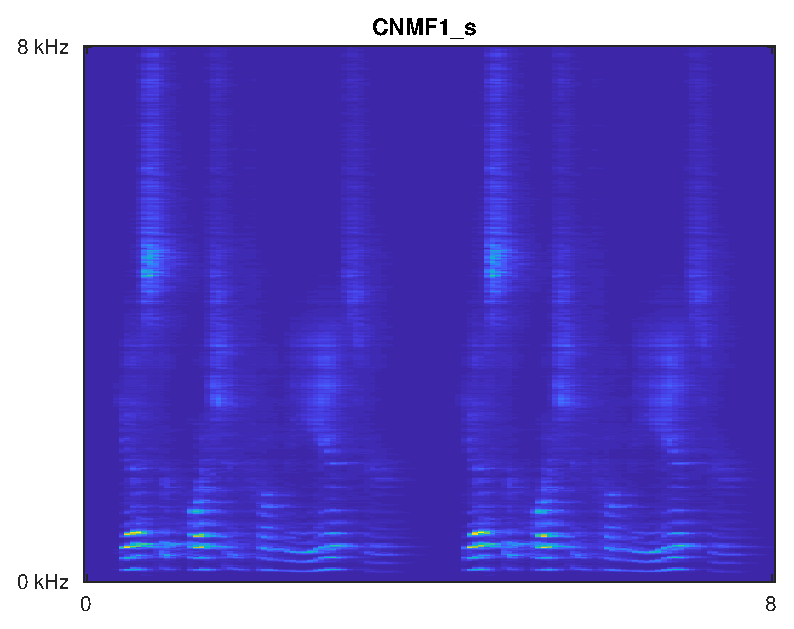
\includegraphics[width = 0.5\linewidth, height = 4cm]{fig/STFT/Sample_mjar0_SI_CNMF1_s_RIR_SimRoom2_far_AnglA.eps}}\\
\subfloat[]{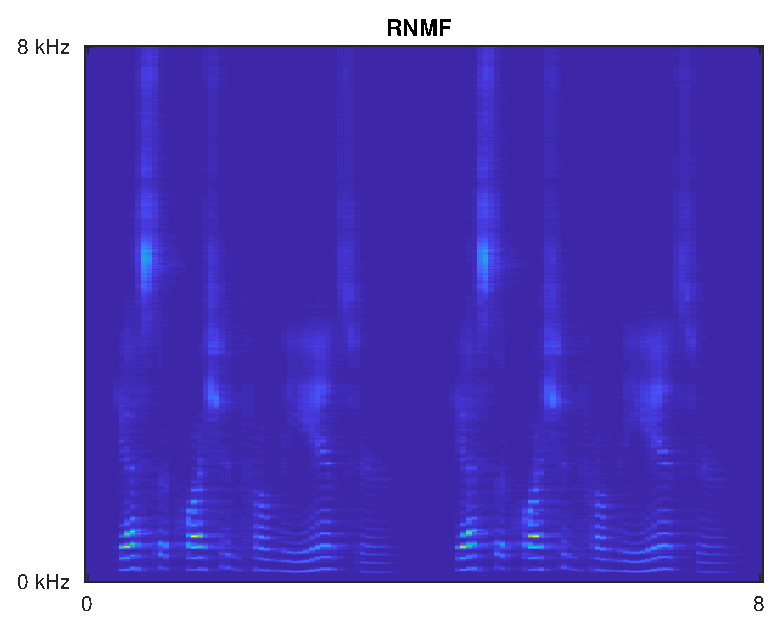
\includegraphics[width = 0.5\linewidth, height = 4cm]{fig/STFT/Sample_mjar0_SI_RNMF_RIR_SimRoom2_near_AnglA.eps}}&
\subfloat[]{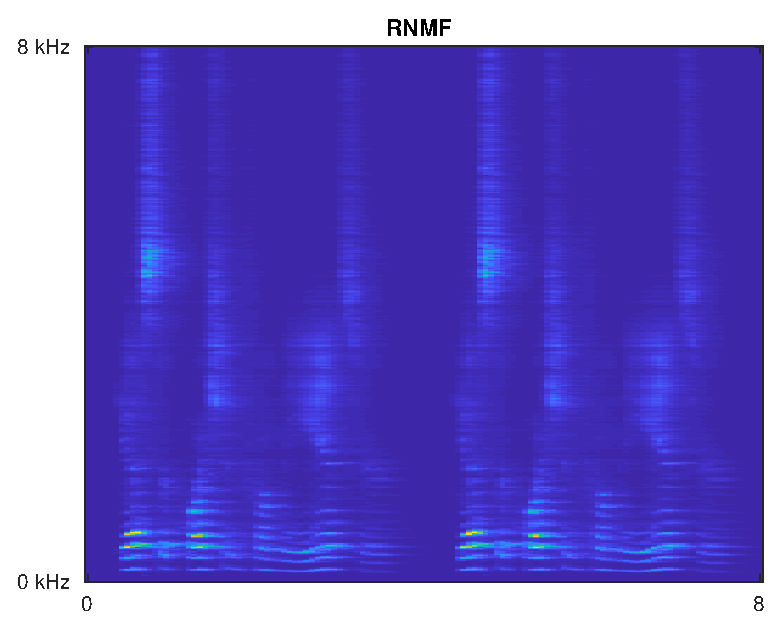
\includegraphics[width = 0.5\linewidth, height = 4cm]{fig/STFT/Sample_mjar0_SI_RNMF_RIR_SimRoom2_far_AnglA.eps}}\\
\end{tabular}
\caption[abc]{Comparison of reverb spectrogram estimated using various reverberation model when SI clean speech bases are used. Models are a smoother version of original spectrogram. The modeling error for all algorithms are small for near case. RNMF is more smoother than CNMF0. Spectrogram estimated using RNMF is mostly same as done by \text{CNMF1\_s}. }
\label{fig:Spectrogram_reverb_with_SI_bases}
\end{figure*}
\fi
% use section* for acknowledgment
\section*{Acknowledgment}
Authors acknowledge the support by Council of Scientific and Industrial
Research (CSIR), India and Tata Consultancy Services (TCS), India

% Can use something like this to put references on a page
% by themselves when using endfloat and the captionsoff option.

%\ifCLASSOPTIONcaptionsoff
%  \newpage
%\fi

%\bibliographystyle{IEEEtran}
%\bibliography{NMF}

\iffalse
\begin{IEEEbiography}{Michael Shell}
Biography text here.
\end{IEEEbiography}

% if you will not have a photo at all:
\begin{IEEEbiographynophoto}{John Doe}
Biography text here.
\end{IEEEbiographynophoto}

% insert where needed to balance the two columns on the last page with
% biographies
%\newpage

#\begin{IEEEbiographynophoto}{Jane Doe}
#Biography text here.
#\end{IEEEbiographynophoto}
\fi

%\end{document}
\fi

